\documentclass[a4paper,12pt]{extreport}

\usepackage[T2A]{fontenc}
\usepackage[utf8]{inputenc}
\usepackage[english,russian]{babel}
\usepackage{tempora}
\usepackage{geometry}
\usepackage{setspace}
\usepackage{indentfirst}
\usepackage{graphicx}
\usepackage{float}
\usepackage{caption}
\usepackage{array}
\usepackage{longtable}
\usepackage{booktabs}
\usepackage{tabularx}
\usepackage{amsmath}
\usepackage{listings}
\usepackage{xcolor}
\usepackage{enumitem}
\usepackage{titlesec}
\usepackage[titles]{tocloft}
\usepackage[hidelinks]{hyperref}
\usepackage{fancyhdr}
\usepackage{needspace}
\usepackage{lastpage}

\geometry{left=30mm,right=15mm,top=20mm,bottom=20mm}
\onehalfspacing
\setlength{\parindent}{1.25cm}
\setlength{\parskip}{0pt}
\AtBeginDocument{%
  \setlength{\abovedisplayskip}{\baselineskip}%
  \setlength{\belowdisplayskip}{\baselineskip}%
  \setlength{\abovedisplayshortskip}{\baselineskip}%
  \setlength{\belowdisplayshortskip}{\baselineskip}%
}
\setlist{nosep,wide=\parindent}
\setlist[itemize]{label=--}
\graphicspath{{images/}}

\titleformat{\chapter}[hang]
  {\normalfont\normalsize\bfseries\filright\hyphenpenalty=10000\exhyphenpenalty=10000}
  {\thechapter}{0.5em}{}
\titleformat{\section}[hang]
  {\normalfont\normalsize\bfseries\filright\hyphenpenalty=10000\exhyphenpenalty=10000}
  {\thesection}{0.5em}{}
\titleformat{\subsection}[hang]
  {\normalfont\normalsize\bfseries\filright\hyphenpenalty=10000\exhyphenpenalty=10000}
  {\thesubsection}{0.5em}{}
\titleformat{name=\chapter,numberless}[block]
  {\normalfont\normalsize\bfseries\filcenter\hyphenpenalty=10000\exhyphenpenalty=10000}
  {}{0pt}{}
\titlespacing{\chapter}{1.25cm}{0pt}{\baselineskip}
\titlespacing{\section}{1.25cm}{\baselineskip}{\baselineskip}
\titlespacing{\subsection}{1.25cm}{\baselineskip}{\baselineskip}
\titlespacing{name=\chapter,numberless}{0pt}{-0.5\baselineskip}{0.5\baselineskip}

\renewcommand{\cftchapleader}{\cftdotfill{\cftdotsep}}
\renewcommand{\cftchapfont}{\normalfont}
\renewcommand{\cftchappagefont}{\normalfont}
\setlength{\cftbeforechapskip}{0pt}
\cftsetindents{chapter}{0em}{1.5em}
\cftsetindents{section}{1em}{2.3em}
\cftsetindents{subsection}{2em}{3.1em}

\captionsetup{labelsep=endash,justification=centering}
\captionsetup[figure]{position=bottom}
\captionsetup[table]{justification=raggedright,singlelinecheck=false,position=top}
\captionsetup[lstlisting]{justification=raggedright,singlelinecheck=false}
\addto\captionsrussian{\renewcommand{\figurename}{Рисунок}}
\addto\captionsrussian{\renewcommand{\tablename}{Таблица}}
\addto\captionsrussian{\renewcommand{\contentsname}{СОДЕРЖАНИЕ}}
\addto\captionsrussian{\renewcommand{\bibname}{СПИСОК ИСПОЛЬЗОВАННЫХ ИСТОЧНИКОВ}}
\makeatletter
\renewcommand{\@biblabel}[1]{#1.}
\makeatother

\fancypagestyle{plain}{%
  \fancyhf{}%
  \fancyfootoffset[L]{15mm}%
  \fancyfoot[C]{\thepage}%
  \renewcommand{\headrulewidth}{0pt}%
}
\pagestyle{plain}

\AtBeginDocument{%
  \setlength{\abovedisplayskip}{\baselineskip}%
  \setlength{\belowdisplayskip}{\baselineskip}%
  \setlength{\abovedisplayshortskip}{\baselineskip}%
  \setlength{\belowdisplayshortskip}{\baselineskip}%
}

\lstdefinestyle{code}{
  basicstyle=\ttfamily\small,
  numbers=left,
  numberstyle=\tiny,
  numbersep=8pt,
  frame=single,
  breaklines=true,
  showstringspaces=false,
  tabsize=4,
  columns=fullflexible,
  inputencoding=utf8,
  extendedchars=true
}

\lstdefinestyle{logstyle}{
  basicstyle=\ttfamily\footnotesize,
  numbers=left,
  numberstyle=\tiny,
  numbersep=7pt,
  xleftmargin=25pt,
  xrightmargin=5pt,
  framexleftmargin=20pt,
  frame=single,
  framesep=4pt,
  breaklines=true,
  breakatwhitespace=false,
  showstringspaces=false,
  showtabs=false,
  tabsize=2,
  columns=fullflexible,
  keepspaces=true,
  inputencoding=utf8,
  extendedchars=true,
  captionpos=t,
  abovecaptionskip=8pt,
  literate={×}{{$\times$}}1
           {«}{{\guillemotleft}}1 {»}{{\guillemotright}}1
           {–}{{\textendash}}1 {—}{{\textemdash}}1 {→}{{$\rightarrow$}}1
           {±}{{$\pm$}}1 {Σ}{{$\Sigma$}}1 {‖}{{$\Vert$}}1 {·}{{$\cdot$}}1
           {…}{{\ldots}}1 {ᵀ}{{\textsuperscript{T}}}1
           {─}{{-}}1 {├}{{|--}}2 {└}{{`--}}2
           {а}{{\char224}}1 {б}{{\char225}}1 {в}{{\char226}}1 {г}{{\char227}}1 {д}{{\char228}}1 {е}{{\char229}}1 {ё}{{\cyryo}}1 {ж}{{\char230}}1 {з}{{\char231}}1 {и}{{\char232}}1 {й}{{\char233}}1 {к}{{\char234}}1 {л}{{\char235}}1 {м}{{\char236}}1 {н}{{\char237}}1 {о}{{\char238}}1 {п}{{\char239}}1 {р}{{\char240}}1 {с}{{\char241}}1 {т}{{\char242}}1 {у}{{\char243}}1 {ф}{{\char244}}1 {х}{{\char245}}1 {ц}{{\char246}}1 {ч}{{\char247}}1 {ш}{{\char248}}1 {щ}{{\char249}}1 {ъ}{{\char250}}1 {ы}{{\char251}}1 {ь}{{\char252}}1 {э}{{\char253}}1 {ю}{{\char254}}1 {я}{{\char255}}1
           {А}{{\char192}}1 {Б}{{\char193}}1 {В}{{\char194}}1 {Г}{{\char195}}1 {Д}{{\char196}}1 {Е}{{\char197}}1 {Ё}{{\CYRYO}}1 {Ж}{{\char198}}1 {З}{{\char199}}1 {И}{{\char200}}1 {Й}{{\char201}}1 {К}{{\char202}}1 {Л}{{\char203}}1 {М}{{\char204}}1 {Н}{{\char205}}1 {О}{{\char206}}1 {П}{{\char207}}1 {Р}{{\char208}}1 {С}{{\char209}}1 {Т}{{\char210}}1 {У}{{\char211}}1 {Ф}{{\char212}}1 {Х}{{\char213}}1 {Ц}{{\char214}}1 {Ч}{{\char215}}1 {Ш}{{\char216}}1 {Щ}{{\char217}}1 {Ы}{{\char219}}1 {Ь}{{\char220}}1 {Э}{{\char221}}1 {Я}{{\char223}}1
}

\newcommand{\code}[1]{\nolinkurl{#1}}
\newcommand{\logfile}[2]{\lstinputlisting[style=logstyle,caption={#1}]{#2}}
\newcommand{\gostappendix}[2][справочное]{%
  \clearpage
  \refstepcounter{chapter}%
  \addcontentsline{toc}{chapter}{Приложение~\thechapter~(#1) #2}%
  {\centering\normalfont\normalsize
    ПРИЛОЖЕНИЕ~\thechapter\par
    (#1)\par
    \bfseries\hyphenpenalty=10000\exhyphenpenalty=10000\relax
    #2\par
  }%
  \nobreak\vspace{\baselineskip}%
}

% Структурный элемент отчёта: заголовок без номера, с записью в содержание.
\newcommand{\structel}[1]{%
  \clearpage\phantomsection\addcontentsline{toc}{chapter}{#1}%
  \chapter*{#1}}

\begin{document}

\begin{titlepage}
\singlespacing
\thispagestyle{empty}
\noindent\begin{minipage}{0.13\textwidth}
  
\includegraphics[width=\linewidth]{b_logo.png}
\end{minipage}%
\hfill%
\begin{minipage}{0.84\textwidth}
\centering\small\bfseries
Министерство науки и высшего образования Российской Федерации\\
Федеральное государственное автономное образовательное учреждение высшего образования\\
<<Московский государственный технический университет имени Н.~Э.~Баумана\\
(национальный исследовательский университет)>>\\
(МГТУ им. Н.~Э.~Баумана)
\end{minipage}

\vspace{0.3cm}
\noindent\rule{\linewidth}{2pt}
\vspace{0.7cm}

\noindent ФАКУЛЬТЕТ \underline{<<Информатика и системы управления>>}\\[0.5cm]
\noindent КАФЕДРА \underline{<<Программное обеспечение ЭВМ и информационные технологии, ИУ7>>}

\vfill
\begin{center}
{\Large\bfseries Лабораторная работа № 3}\\[0.4cm]
{\large по дисциплине}\\[0.2cm]
{\large\bfseries <<Программирование (специальные главы)>>}\\[1cm]
{\large\bfseries Сравнение больших языковых моделей при разработке системы попарного сравнения текстовых документов}
\end{center}
\vfill

\noindent\textbf{Студент:} \underline{Логинов Виктор Николаевич}\\[0.5cm]
\noindent\textbf{Группа:} \underline{СГН3-11М}\\[0.5cm]
\noindent\textbf{Преподаватель:} \underline{Строганов Юрий Владимирович}

\vfill
\begin{center}
Москва 2026
\end{center}
\end{titlepage}
\setcounter{page}{2}

\structel{РЕФЕРАТ}

Отчет \pageref{LastPage}~с., 33~рис., 4~табл., 11~источн., 6~прил.

{\noindent\raggedright\hyphenpenalty=10000\exhyphenpenalty=10000\relax
ПОПАРНОЕ СРАВНЕНИЕ ДОКУМЕНТОВ, TF--IDF, BGE-M3, МЕРЫ БЛИЗОСТИ, ROC AUC, БОЛЬШИЕ ЯЗЫКОВЫЕ МОДЕЛИ, PYTHON\par}

Объектом исследования являются четыре реализации системы попарного сравнения текстовых документов, созданные GigaChat, Qwen3.7-Plus, Korolev AI и DeepSeek.

Цель работы --- экспериментально оценить способность больших языковых моделей создавать воспроизводимый программный комплекс, который читает документы TXT, HTML, DOCX и ODT, строит три представления корпуса, вычисляет одиннадцать мер близости и формирует результаты, пригодные для анализа.

Методами исследования служат единый исходный запрос, автоматическая приёмка на пустом, вырожденном, малом и полном корпусе, проверка структуры матриц, диапазонов и диагоналей, а также метрик ROC AUC и average precision.

В результате работы все четыре реализации обработали 50 документов и сформировали 33 матрицы и 40425 строк пар; принятые версии получены на шестой, четвёртой, четвёртой и третьей итерациях. Наибольший ROC AUC 0,953218 и наименьшее время полного запуска 7,06~с показала реализация Qwen3.7-Plus.

Область применения --- сравнительный анализ текстов и контроль генеративного программирования.

\clearpage

\tableofcontents
\clearpage

\chapter*{ПЕРЕЧЕНЬ СОКРАЩЕНИЙ И ОБОЗНАЧЕНИЙ}
\addcontentsline{toc}{chapter}{ПЕРЕЧЕНЬ СОКРАЩЕНИЙ И ОБОЗНАЧЕНИЙ}

В настоящем отчёте о лабораторной работе применяют следующие сокращения и обозначения.

\noindent
\begin{tabularx}{\linewidth}{@{}l@{\quad---\quad}X@{}}
БЯМ & большая языковая модель \\
AP & средняя точность (average precision) \\
BGE-M3 & модель эмбеддингов BAAI/bge-m3 \\
CSV & текстовый формат табличных данных с разделителями \\
CUDA & платформа параллельных вычислений NVIDIA \\
DOCX & формат текстового документа Office Open XML \\
GPU & графический процессор \\
HTML & язык гипертекстовой разметки \\
NaN & неопределённое числовое значение (Not a Number) \\
ODT & формат текстового документа OpenDocument \\
ROC AUC & площадь под кривой рабочих характеристик \\
TF--IDF & частота терма, взвешенная обратной частотой по документам \\
TXT & файл с простым текстом
\end{tabularx}

\chapter*{ВВЕДЕНИЕ}
\addcontentsline{toc}{chapter}{ВВЕДЕНИЕ}

Цель работы --- экспериментально оценить способность больших языковых моделей создавать воспроизводимый программный комплекс для попарного сравнения текстовых документов. Модель должна не только написать запускаемый код, но и корректно извлечь тексты из нескольких форматов, построить три представления корпуса, вычислить единый набор мер близости, сохранить промежуточные данные и сформировать результаты, пригодные для последующего анализа.

В исследовании сопоставлены GigaChat, Qwen3.7-Plus, Korolev AI и DeepSeek. Каждой модели передавалась одна и та же постановка задачи. Требовалось подготовить решение на Python, которое обрабатывает документы TXT, HTML, DOCX и ODT, строит представления на основе мешка слов, TF--IDF по леммам и эмбеддингов BGE-M3, а затем вычисляет для каждой пары документов одиннадцать мер.

Результат проверялся на нескольких уровнях. Сначала контролировались синтаксис программы, состав зависимостей и поведение на пустом каталоге. Затем применялись малые наборы с пустыми и непустыми документами. После этого решение запускалось на полном корпусе из 50 документов семи тематических групп. Итог принимался только при наличии 33 квадратных матриц, корректных диагоналей и диапазонов, полного длинного набора пар, ближайших соседей, сводных метрик качества, визуализаций и метаданных запуска.

Актуальность работы обусловлена тем, что уверенное текстовое описание модели не гарантирует вычислительную корректность результата. Ошибки проявлялись в чтении ODT, обработке пустого словаря, выборе устройства, интерпретации расстояний и сходств, а также в применении взвешенных коэффициентов Жаккара и Дайса к знаковым эмбеддингам. Часть дефектов обнаруживалась только при фактическом запуске и проверке числовых инвариантов.

Объектом исследования являются последовательности ответов четырёх БЯМ при решении одной задачи. Предмет исследования --- корректность, полнота и устойчивость создаваемых ими программных реализаций. Под устойчивостью понимается способность устранить обнаруженный дефект без потери уже работающих частей и без нарушения общего контракта выходных данных.

Для достижения цели формулировался единый запрос, сохранялись исходные ответы моделей, из них извлекались файлы программы и зависимостей, выполнялись автоматические проверки, формировались исправляющие запросы и повторялись испытания. После получения принятой версии сравнивались число итераций, характер ошибок, размерность представлений, время полного запуска и качество разделения тематически близких и далёких пар.

Практический результат работы состоит в получении четырёх независимых реализаций одного программного комплекса и воспроизводимого процесса их проверки. Сохранённые цепочки позволяют оценить не только финальный код, но и объём сопровождения, который потребовался для его доведения до заданного состояния.

\chapter{Аналитическая часть}

\section{Описание задачи и выбранных инструментов}

\subsection{Корпус документов и представления текста}

Исходный корпус содержит 50 документов, распределённых по семи тематическим каталогам: <<Анамнез>>, <<Биохимия крови>>, <<Комментаторы>>, <<Неорганическая химия>>, <<Органическая химия>>, <<Спортивная медицина>> и <<Ставки на спорт>>. В набор входят файлы TXT, HTML, DOCX и ODT. Имя родительского каталога используется как тематическая метка при оценке качества, но не передаётся алгоритму построения признаков.

Для каждого документа требовалось построить три представления. Первое --- абсолютные частоты словоформ после приведения к нижнему регистру и очистки текста. Второе --- разреженная TF--IDF-матрица по нормальным формам слов, полученным морфологическим анализатором. Третье --- плотный вектор BGE-M3~\cite{bge-m3} размерности 1024, формируемый для фрагментов документа и агрегируемый в единое представление.

\Needspace{14\baselineskip}
TF--IDF вычисляется по формуле~\eqref{eq:tfidf}
\begin{equation}
\label{eq:tfidf}
\operatorname{tfidf}(t,d)=\operatorname{tf}(t,d)\log\frac{N+1}{\operatorname{df}(t)+1},
\end{equation}

где $\operatorname{tfidf}(t,d)$ --- вес терма $t$ в документе $d$;\\
\phantom{где }$t$ --- терм;\\
\phantom{где }$d$ --- документ;\\
\phantom{где }$\operatorname{tf}(t,d)$ --- частота терма $t$ в документе $d$;\\
\phantom{где }$N$ --- число документов корпуса;\\
\phantom{где }$\operatorname{df}(t)$ --- число документов, содержащих этот терм.

Сглаживание исключает деление на ноль, а нормировка делает документы различной длины сопоставимыми.

\Needspace{17\baselineskip}
\subsection{Меры попарной близости}

Для каждого представления вычислялись косинусная близость, корреляции Пирсона и Спирмена, взвешенные коэффициенты Жаккара и Дайса, а также манхэттенское, евклидово и чебышёвское расстояния. Для трёх расстояний дополнительно строилась монотонная мера близости по формуле~\eqref{eq:distance}
\begin{equation}
\label{eq:distance}
s(d)=\frac{1}{1+d},
\end{equation}

где $s(d)$ --- близость, соответствующая расстоянию $d$;\\
\phantom{где }$d$ --- неотрицательное расстояние между векторами.

Таким образом, для каждого представления формировалось одиннадцать матриц, а суммарно --- 33 матрицы размера $N\times N$.

\Needspace{13\baselineskip}
Косинусная близость двух векторов $x$ и $y$ определяется по формуле~\eqref{eq:cosine}
\begin{equation}
\label{eq:cosine}
s_{\cos}(x,y)=\frac{x^{T}y}{\|x\|_2\|y\|_2},
\end{equation}

где $s_{\cos}(x,y)$ --- косинусная близость векторов;\\
\phantom{где }$x$, $y$ --- векторы признаков сравниваемых документов;\\
\phantom{где }$x^{T}y$ --- скалярное произведение векторов;\\
\phantom{где }$\|x\|_2$, $\|y\|_2$ --- их евклидовы нормы.

\Needspace{13\baselineskip}
Взвешенный коэффициент Жаккара для неотрицательных векторов вычисляется по формуле~\eqref{eq:jaccard}
\begin{equation}
J(x,y)=\frac{\sum_k\min(x_k,y_k)}{\sum_k\max(x_k,y_k)}, \label{eq:jaccard}
\end{equation}

где $J(x,y)$ --- взвешенный коэффициент Жаккара;\\
\phantom{где }$x$, $y$ --- неотрицательные векторы одинаковой размерности;\\
\phantom{где }$k$ --- индекс координаты, суммирование охватывает все координаты;\\
\phantom{где }$x_k$, $y_k$ --- координаты соответствующих векторов;\\
\phantom{где }$\min$, $\max$ --- выбор меньшего и большего из двух значений.

\Needspace{12\baselineskip}
Взвешенный коэффициент Дайса вычисляется по формуле~\eqref{eq:dice}
\begin{equation}
D(x,y)=\frac{2\sum_k\min(x_k,y_k)}{\sum_k(x_k+y_k)}, \label{eq:dice}
\end{equation}

где $D(x,y)$ --- взвешенный коэффициент Дайса;\\
\phantom{где }$x$, $y$ --- неотрицательные векторы одинаковой размерности;\\
\phantom{где }$k$ --- индекс координаты;\\
\phantom{где }$x_k$, $y_k$ --- координаты соответствующих векторов;\\
\phantom{где }$\min$ --- выбор меньшего из двух значений.

\Needspace{13\baselineskip}
Компоненты BGE-M3 могут быть отрицательными, поэтому непосредственное применение этих формул способно дать значения вне диапазона $[0;1]$. В окончательной методике только для Жаккара и Дайса использовалось преобразование~\eqref{eq:signed-split}
\begin{equation}
\label{eq:signed-split}
x_{\mathrm{overlap}}=[\max(x,0);\max(-x,0)],
\end{equation}

где $x_{\mathrm{overlap}}$ --- неотрицательное представление удвоенной размерности;\\
\phantom{где }$x$ --- исходный знаковый вектор эмбеддинга;\\
\phantom{где }$\max(x,0)$ --- покомпонентный максимум координат $x$ и нуля;\\
\phantom{где }$\max(-x,0)$ --- покомпонентный максимум координат $-x$ и нуля;\\
\phantom{где }$[\,\cdot\,;\,\cdot\,]$ --- последовательное объединение двух векторов.

Оно разносит положительную и отрицательную части в разные неотрицательные координаты. Косинус, корреляции и расстояния при этом вычисляются по исходному знаковому вектору, что сохраняет их смысл.

\subsection{Форматы результатов и критерии приёмки}

Программа должна сохранять список документов и извлечённые тексты, разреженные и плотные векторы, отдельные CSV-матрицы, длинную таблицу всех пар, ближайших соседей, сводку качества, три тепловые карты и метаданные запуска. Имена файлов могли незначительно различаться, если их назначение оставалось однозначным и проверяемым.

Критерии приёмки выводились из контракта задачи. Матрицы обязаны быть квадратными и симметричными, не содержать NaN и бесконечностей; диагональ сходств равна единице, диагональ расстояний --- нулю. Взвешенные коэффициенты Жаккара и Дайса должны находиться в $[0;1]$. Для пустого входного каталога программа не должна загружать BGE-M3 и аварийно завершаться. Если тематические метки образуют только один класс пар, ROC AUC и average precision заменяются оговорённым нейтральным значением $0{,}5$.

\section{Характеристика используемых БЯМ}

\subsection{GigaChat}

GigaChat~\cite{gigachat} использовался в гостевом режиме. Модель предоставила цельный вариант программы и активно дополняла его после получения отчётов проверок. Первые ответы содержали ошибки в структуре сводки качества, классификации расстояний, обработке пустого корпуса и выборе ближайших соседей. Позднее потребовалось уточнить режим выбора устройства, заголовки CSV и методику работы со знаковыми эмбеддингами.

Сильной стороной модели стала способность последовательно устранять перечисленные дефекты. Однако первая реализация signed-split содержала синтаксическую ошибку и неверную ось конкатенации, поэтому окончательный вариант был принят только на шестой итерации.

\subsection{Qwen3.7-Plus}

Qwen3.7-Plus~\cite{qwen} использовался без входа в учётную запись; возрастное подтверждение было выполнено пользователем вручную. Начальный ответ охватывал большую часть требований, но не выдерживал пустой корпус, пустой TF--IDF-словарь, отдельные HTML-случаи и фактическую работу с CUDA. После второго ответа основная функциональность стала работоспособной.

На третьей итерации модель описала правильное преобразование знакового вектора, однако фактически не внесла его в код. Это различие между пояснением и реализацией было обнаружено проверкой диапазонов. Четвёртая версия содержала реальное преобразование и прошла полный набор испытаний.

\subsection{Korolev AI}

Работа с Korolev AI~\cite{korolev} выполнялась пользователем вручную. Первые варианты неверно извлекали ODT, не реализовывали signed-split и неполно обрабатывали пустой корпус. После исправления способ извлечения ODT всё ещё обращался к отсутствующей функции, что обнаружилось только на полном наборе форматов.

Третья версия прошла полный корпус, но возвращала неопределённый ROC AUC на наборе из двух пустых документов с одной тематической меткой. После явного требования нейтрального значения $0{,}5$ четвёртая версия была принята.

\subsection{DeepSeek}

Первый ответ DeepSeek~\cite{deepseek} был получен на усечённый запрос и потому создавал проект с иной схемой признаков. После передачи полной постановки вторая итерация приблизилась к требуемому контракту, но содержала неверный способ чтения ODT, отличающиеся имена признаковых файлов и широкую, а не длинную, таблицу пар.

Третья версия исправила эти расхождения и прошла все испытания. Одна неполная копия ответа второй итерации была сохранена как технический артефакт захвата, но не учитывалась как самостоятельная итерация. Доступ к официальному чату потребовал входа в учётную запись, хотя в исходных условиях сервиса ожидался режим без регистрации; это ограничение фиксируется как свойство фактического процесса.

\section{Сравнительный анализ выбранных БЯМ}

Все четыре модели смогли сформировать работоспособный программный комплекс, но ни один первый ответ не был принят без исправлений. Общими источниками ошибок стали граничные случаи, многокомпонентные форматы документов и различие между математически допустимой операцией и требуемой интерпретацией метрики.

До выполнения эксперимента нельзя было считать одну модель заведомо лучшей. Итоговая оценка учитывала три группы свойств. Первая относится к полноте реализации: охват форматов, представлений, матриц и артефактов. Вторая характеризует вычислительную корректность: диапазоны, диагонали, симметрию, отсутствие неопределённых значений и обработку пустых наборов. Третья отражает практическую эффективность: число ответов до приёмки, локальность исправлений и время выполнения принятой программы.

Особое значение имело различие между текстом ответа и поведением программы. Модель могла уверенно сообщить о поддержке CUDA, ODT или signed-split, однако при запуске соответствующая ветвь не выполнялась либо завершалась ошибкой. Поэтому сравнение строилось по сохранённым файлам и фактическим результатам, а не по самоописанию модели.

\chapter{Конструкторский раздел}

\section{Процесс взаимодействия с моделями}

Всем моделям передавалась единая постановка. Исходный запрос задавал интерфейс командной строки, форматы документов, правила очистки и лемматизации, три представления, перечень мер, структуру выходного каталога и граничные случаи.

Codex выполнял роль внутреннего контроллера экспериментального процесса и организовывал всю техническую приёмку решений больших языковых моделей. Он получал ответы GigaChat, Qwen3.7-Plus и DeepSeek. Обмен с Korolev AI вёл пользователь, после чего ответ включался в тот же цикл обработки и проверки. Для каждой итерации Codex сохранял исходный ответ, извлекал \code{solution.py} и \code{requirements.txt} и связывал их с каталогом результатов и протоколом испытаний. Первоначальный код и исправленные версии создавали исследуемые модели.

Codex управлял последовательностью допуска версии к испытаниям. Сначала он проверял синтаксис командой \code{py_compile}, затем запускал программу на пустом каталоге, двух пустых документах одной категории и смешанном наборе из шести документов. После этих этапов выполнялся запуск на полном корпусе из 50 документов. Малые наборы позволяли выявить ошибки импорта, пустого словаря и структуры таблиц до полного вычисления матриц. Результаты каждого этапа становились основанием для продолжения приёмки либо возврата модели конкретного замечания.

После каждого прогона Codex запускал валидатор \code{tests/verify_output.py}, проверявший комплектность файлов, конечность чисел, диапазоны значений, симметрию и диагонали матриц. Допуск охватывал все три представления, одиннадцать мер и преобразований расстояний в близость, единый порядок документов и согласованность выходных таблиц. По результатам неудачного теста Codex фиксировал наблюдаемый дефект и составлял корректирующий запрос с условием, которому должна удовлетворять новая версия.

При получении исправления Codex сопоставлял новую версию с замечанием и повторял ранее успешные сценарии. Финальное решение о технической приёмке принималось им по совокупности проверок на малых наборах и полном корпусе. С итоговой версией связывались принятый код, результаты запуска и протокол валидатора. Таким образом, вся операционная работа с ответами и их приёмка проходили через Codex, от извлечения программы до допуска результатов к сравнительному анализу и визуализации.

\section{Построение исправляющего промта}

Исправляющий запрос строился по принципу минимальной проверяемой правки. Вместо общей формулировки <<исправь программу>> указывались конкретный сценарий запуска, сообщение об ошибке или неверный диапазон, ожидаемый состав файлов и правило, которое должно выполняться после изменения.

Для числовых дефектов в запрос включалась математическая причина. Так, отрицательные компоненты BGE-M3 не предлагалось обнулять: это уничтожило бы часть информации. Модели передавалось точное правило разбиения знакового вектора на положительную и отрицательную части, а также запрет применять преобразование к косинусу, корреляциям и расстояниям.

Отдельно требовалось сохранять воспроизводимость. Исправление не должно было удалять метаданные, менять интерфейс командной строки или заменять длинную таблицу пар набором несвязанных файлов. Такой подход позволял оценивать устойчивость: если локальная правка разрушала ранее пройденный тест, следующая версия не принималась.

\section{Проектирование набора проверок}

Набор проверок проектировался как последовательность от дешёвых к полным. Статическая стадия проверяла синтаксис и импорты. Пустой каталог контролировал ранний выход без загрузки BGE-M3. Набор из двух пустых документов проверял матрицы размерности $2\times2$, отсутствие признаков и поведение метрик при одном классе пар. Смешанный набор из шести документов выявлял ошибки форматов, разреженных матриц и ближайших соседей.

Полный запуск подтверждал обработку всех 50 документов и создание 33 матриц. Для каждой матрицы контролировались форма, симметрия, конечность элементов и диагональ. Для мер сходства проверялся допустимый диапазон. Таблица всех пар должна была содержать $1225\cdot33=40425$ строк, поскольку для 50 документов существует $50\cdot49/2=1225$ неупорядоченных пар.

Наконец, сводка качества проверялась по тематическим меткам. Для каждой меры вычислялись средние значения внутри и между темами, ROC AUC и average precision. Эти показатели использовались не для доказательства универсального превосходства реализации, а для подтверждения того, что числовые результаты связаны с содержанием корпуса.

\chapter{Технологическая часть}

\section{Выбор языка и среды программирования}

Все модели использовали Python. Язык выбран благодаря библиотекам для чтения документов, морфологического анализа, разреженных матриц, машинного обучения и нейросетевых эмбеддингов. Испытания выполнялись в изолированной виртуальной среде Python 3.12 под Windows 11.

Для числовых операций применялись NumPy, SciPy, pandas и scikit-learn~\cite{sklearn}; для русского морфологического анализа --- pymorphy3~\cite{pymorphy3}; для DOCX и ODT --- python-docx~\cite{docx} и odfpy~\cite{odfpy}; для HTML --- BeautifulSoup~\cite{bs4}. Эмбеддинги формировались моделью BGE-M3 через transformers~\cite{transformers} или sentence-transformers. Полные запуски выполнялись на GPU NVIDIA GeForce RTX 4070 Ti SUPER; кэш модели был общим для всех решений.

\section{Реализация программного обеспечения}

\subsection{Решение GigaChat}

Принятая версия разделяет чтение документов, построение признаков, вычисление матриц и сохранение результатов. Для BGE-M3 используется выбор устройства \code{auto/cpu/cuda} и обработка документов фрагментами. Полный запуск сформировал матрицы размерности $50\times7165$ для мешка слов, $50\times4480$ для TF--IDF и $50\times1024$ для BGE-M3.

\subsection{Решение Qwen3.7-Plus}

Qwen организовал программу как единый файл с явными функциями извлечения, нормализации, построения представлений и расчёта метрик. В принятом каталоге фактические размерности составили $50\times7555$, $50\times4645$ и $50\times1024$. Отличие словарей от других решений связано с деталями токенизации и фильтрации, которые не были полностью унифицированы исходным запросом.

\subsection{Решение Korolev AI}

Решение Korolev AI использует sentence-transformers для BGE-M3 и явно фиксирует правила для пустых и вырожденных векторов. Итоговые размерности составили $50\times7549$, $50\times4633$ и $50\times1024$. В метаданных отдельно сохранены правило signed-split и подстановка $0{,}5$ для неопределимых AUC и AP.

\subsection{Решение DeepSeek}

DeepSeek сформировал длинную таблицу с отдельной строкой для каждой комбинации пары, представления и метрики. В результате \code{all_pairs.csv} содержит 40425 строк. Размерности представлений равны $50\times7497$, $50\times4473$ и $50\times1024$. Метаданные подробно фиксируют правила обработки нулевых строк, константных векторов и неопределённых метрик.

\section{Протоколы взаимодействия с БЯМ}

\subsection{Протокол GigaChat}

Полный протокол приведён в приложении~\ref{app:gigachat}.

Цепочка GigaChat состояла из шести ответов. Первая версия не выдерживала ряд структурных и граничных проверок. В следующих версиях были исправлены сводка качества, интерпретация расстояний, пустой вход, ближайшие соседи и параметры запуска. Пятая версия содержала дефект в реализации signed-split; шестая прошла пустой, малый и полный сценарии.

\subsection{Протокол Qwen3.7-Plus}

Полный протокол приведён в приложении~\ref{app:qwen}.

Qwen потребовал четыре ответа. После устранения ошибок пустого корпуса и чтения документов третий ответ формально заявлял нужную методику, но не реализовывал её в вычислительной ветви. Четвёртая версия устранила расхождение и была принята после полного повторного прогона.

\subsection{Протокол Korolev AI}

Полный протокол приведён в приложении~\ref{app:korolev}.

Korolev AI потребовал четыре ответа. Две первые итерации отклонены из-за ODT и граничных случаев. Третья корректно выполнила полный корпус, но не прошла сценарий с одним классом тематических пар. Четвёртая версия задала нейтральные значения для неопределимых метрик и прошла все испытания.

\subsection{Протокол DeepSeek}

Полный протокол приведён в приложении~\ref{app:deepseek}.

DeepSeek потребовал три учитываемых ответа. Первый относился к усечённой постановке и не соответствовал требуемой архитектуре. Во второй версии оставались ошибки ODT и структуры результатов. Третья версия исправила контракт и была принята. Неполный технический захват второй версии не считался новым ответом и сохранён отдельно только для прозрачности архива.

Исходный код финальных решений приведён в приложении~\ref{app:code}. Состав электронного приложения описан в приложении~\ref{app:electronic}.

\chapter{Исследовательский раздел}

\section{Объекты исследования и методика оценки}

Объектами исследования являлись четыре полные цепочки <<исходный запрос --- ответ --- запуск --- корректирующий запрос>>. Финальные программы запускались в одной среде, на одном корпусе и с общим кэшем BGE-M3. Такой порядок уменьшает влияние загрузки модели и различий аппаратного обеспечения, хотя не устраняет различия внутренней реализации.

Практическая эффективность оценивалась по числу ответов до приёмки и времени полного запуска. Числовое качество оценивалось по ROC AUC и average precision при разделении пар на внутритематические и межтематические. Для каждой реализации также фиксировались размерности признаков и диапазоны взвешенных коэффициентов на BGE-M3.

\section{Ход исследования и анализ взаимодействия}

\subsection{GigaChat}

GigaChat потребовал наибольшее число итераций --- шесть. Основная причина состояла не в отсутствии общей архитектуры, а в последовательном проявлении независимых дефектов. После исправления структуры результата появились требования к устройству и CSV, а после введения signed-split --- синтаксическая и размерностная ошибки. Модель смогла завершить задачу, но стоимость сопровождения оказалась максимальной.

\subsection{Qwen3.7-Plus}

Qwen завершил работу за четыре итерации и показал наибольшее значение ROC AUC среди принятых реализаций. В третьем ответе модель описала signed-split, но при проверке шести документов валидатор обнаружил значение взвешенного коэффициента Жаккара около $-1{,}58629$ при допустимом диапазоне $[0;1]$. Codex установил, что в расчёт по-прежнему попадали исходные знаковые координаты, и зафиксировал причину отклонения итерации. В четвёртой версии преобразование было реализовано, а повторный прогон подтвердил соблюдение диапазона.

\subsection{Korolev AI}

Korolev AI также потребовал четыре итерации. Третья версия прошла проверку на 50 документах, однако при проверке двух пустых документов одной тематики все 24 значения ROC AUC оказались неопределёнными. Codex включил в корректирующий запрос требование присваивать обеим оценкам качества документированное значение $0{,}5$, если все пары относятся к одному классу. Четвёртая версия прошла и этот тест, и повторную проверку полного корпуса.

\subsection{DeepSeek}

DeepSeek завершил цепочку за три учитываемых ответа. После получения полной постановки исправления были достаточно локальными, а итоговая версия подробно документировала граничные правила. При этом первая итерация показывает чувствительность результата к полноте исходного запроса: модель сформировала правдоподобный, но иной проект, когда часть контракта не была передана.

\section{Сравнительный анализ результатов}

В таблице~\ref{tab:iterations} приведено число ответов до приёмки. Техническая неполная копия ответа DeepSeek не включена, поскольку не являлась новой генерацией модели.

\begin{table}[H]
\raggedright
\caption{Количество ответов до принятой версии}
\label{tab:iterations}
\begin{tabular}{|l|c|c|}
\hline
\multicolumn{1}{|c|}{Модель} & Число ответов & Принятая итерация \\
\hline
GigaChat & 6 & 06 \\
\hline
Qwen3.7-Plus & 4 & 04 \\
\hline
Korolev AI & 4 & 04 \\
\hline
DeepSeek & 3 & 03 \\
\hline
\end{tabular}
\end{table}

Размерности признаковых пространств представлены в таблице~\ref{tab:shapes}. Все реализации получили одинаковое число документов и одинаковую размерность BGE-M3, но словари мешка слов и лемм различаются. Следовательно, даже при общей постановке остаются допустимые степени свободы в токенизации, очистке и морфологической фильтрации.

\begin{table}[H]
\raggedright
\caption{Размерности финальных представлений}
\label{tab:shapes}
\begin{tabular}{|l|c|c|c|}
\hline
\multicolumn{1}{|c|}{Модель} & Мешок слов & TF--IDF & BGE-M3 \\
\hline
GigaChat & $50\times7165$ & $50\times4480$ & $50\times1024$ \\
\hline
Qwen3.7-Plus & $50\times7555$ & $50\times4645$ & $50\times1024$ \\
\hline
Korolev AI & $50\times7549$ & $50\times4633$ & $50\times1024$ \\
\hline
DeepSeek & $50\times7497$ & $50\times4473$ & $50\times1024$ \\
\hline
\end{tabular}
\end{table}

Сводные показатели качества приведены в таблице~\ref{tab:quality}. Во всех случаях лучшими оказались меры по BGE-M3. Максимальное значение $0{,}953218$ получено решением Qwen для косинуса, корреляции Пирсона и преобразованного евклидова расстояния. Результаты Korolev AI и DeepSeek почти совпадают, что объясняется близкой схемой обработки BGE-M3, однако их словарные представления и программная структура различаются.

\begin{table}[H]
\raggedright
\caption{Лучшие ROC AUC финальных решений}
\label{tab:quality}
\small
\begin{tabularx}{\textwidth}{|l|>{\raggedright\arraybackslash}X|c|c|}
\hline
\multicolumn{1}{|c|}{Модель} & \multicolumn{1}{c|}{Лучшая комбинация} & Лучший ROC AUC & ROC AUC Жаккара/Дайса \\
\hline
GigaChat & BGE-M3, Спирмен & 0,915033 & 0,912474 \\
\hline
Qwen3.7-Plus & BGE-M3, косинус / Пирсон / евклидова близость & 0,953218 & 0,945851 \\
\hline
Korolev AI & BGE-M3, Спирмен & 0,943656 & 0,942395 \\
\hline
DeepSeek & BGE-M3, Спирмен & 0,943644 & 0,942395 \\
\hline
\end{tabularx}
\end{table}

После signed-split все значения взвешенных мер оказались в требуемом диапазоне. Минимумы Жаккара составили 0,230147 для GigaChat, 0,286407 для Qwen и 0,225772 для Korolev AI и DeepSeek; максимумы во всех случаях равны единице. Для Дайса соответствующие минимумы равны 0,374178, 0,445283 и 0,368375.

Визуальное сопоставление всех мер для трёх представлений приведено в разделе~\ref{sec:all-measures}.

\subsection*{Производительность и метрики получения результата}
\addcontentsline{toc}{subsection}{Производительность и метрики получения результата}

Время полного запуска измерялось самими программами после загрузки модели из локального кэша. GigaChat завершил вычисления примерно за 11,77~с, Qwen --- за 7,06~с, Korolev AI --- за 17,71~с, DeepSeek --- за 15,18~с. Эти значения характеризуют конкретные реализации, а не скорость генерации ответов сервисами.

На время влияли используемая библиотека BGE-M3, схема пакетной обработки, повторная загрузка модели и организация сохранения 33 матриц. Поэтому небольшое время Qwen нельзя напрямую интерпретировать как преимущество самой БЯМ. Более корректно рассматривать его как свойство созданного ею кода в зафиксированной среде.

Сочетание числа ответов и времени выполнения даёт два независимых измерения практической эффективности. DeepSeek потребовал меньше циклов взаимодействия, но его программа выполнялась дольше Qwen. GigaChat работал достаточно быстро, однако потребовал больше исправляющих запросов. Ни одна отдельная величина не описывает качество результата полностью.

\clearpage
\section{Визуальное сопоставление всех мер близости}
\label{sec:all-measures}

Для каждой из трёх систем признаков представлены все одиннадцать матриц, полученных в финальных запусках. Всего приведены 33 сравнительных рисунка, каждый из которых содержит четыре панели в порядке GigaChat, Qwen3.7-Plus, Korolev AI и DeepSeek. Таким образом, визуальное сравнение охватывает 132 матрицы по 50 документам.

Изображения построены по CSV-файлам принятых реализаций, сохранённым в подкаталоге \code{final/output/matrices} каждой модели. Перед построением Codex проверил комплектность всех 132 матриц, соответствие строк и столбцов документам корпуса и конечность значений. Для сравнения матрицы приведены к одному порядку, полученному сортировкой относительных путей документов. Индексы на осях соответствуют тематическим группам из таблицы~\ref{tab:heatmap-groups}. Линии внутри панелей показывают границы этих групп.

\begin{table}[H]
\caption{Тематические группы в порядке документов на тепловых картах}
\label{tab:heatmap-groups}
\centering
\begin{tabular}{|c|l|}
\hline
Индексы документов & Тематика \\
\hline
1--8 & Анамнез \\
9--15 & Биохимия крови \\
16--22 & Комментаторы \\
23--29 & Неорганическая химия \\
30--36 & Органическая химия \\
37--43 & Спортивная медицина \\
44--50 & Ставки на спорт \\
\hline
\end{tabular}
\end{table}

В пределах каждого рисунка все четыре панели используют одну цветовую шкалу. Для косинусной близости и корреляций Пирсона и Спирмена выбран диапазон $[-1;1]$. Для взвешенных коэффициентов Жаккара и Дайса и трёх близостей, полученных из расстояний по формуле~\eqref{eq:distance}, используется диапазон $[0;1]$. У этих показателей большему значению соответствует большая близость.

Для исходных расстояний шкала начинается с нуля и заканчивается общим максимумом по четырём моделям в данном представлении. Меньшее расстояние соответствует большей близости. Под названием модели указан фактический диапазон значений её матрицы, что позволяет оценить различия масштаба при общей шкале. Различия между исходным расстоянием и его преобразованием в близость видны на отдельных рисунках.

\clearpage
\subsection{Представление на основе мешка слов}

Матрицы косинусной близости для данного представления приведены на рисунке~\ref{fig:all-count-bow-cosine}.

\begin{figure}[H]
\centering
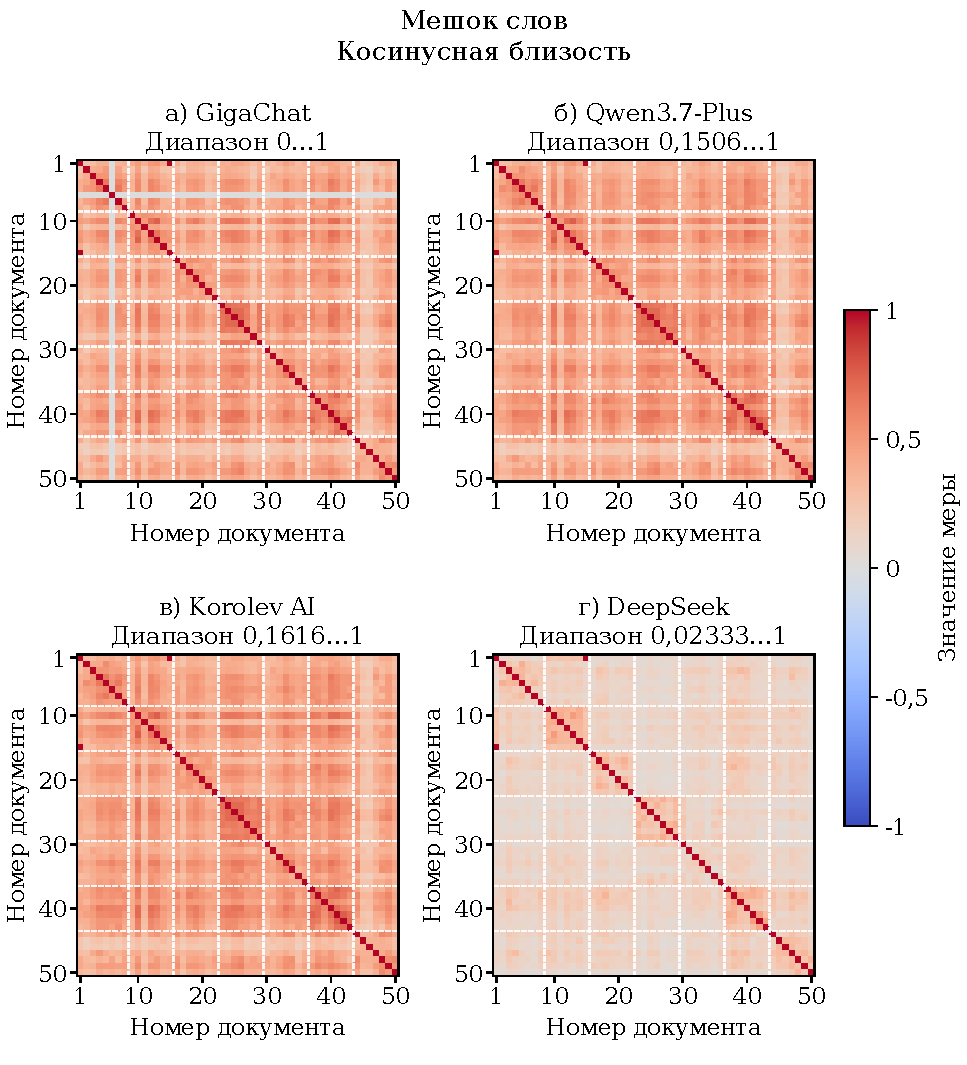
\includegraphics[width=\linewidth,height=0.78\textheight,keepaspectratio]{comparison_count_bow_cosine.pdf}
\caption{Косинусная близость для представления мешка слов}
\label{fig:all-count-bow-cosine}
\end{figure}
\clearpage

Матрицы корреляции Пирсона для данного представления приведены на рисунке~\ref{fig:all-count-bow-pearson}.

\begin{figure}[H]
\centering
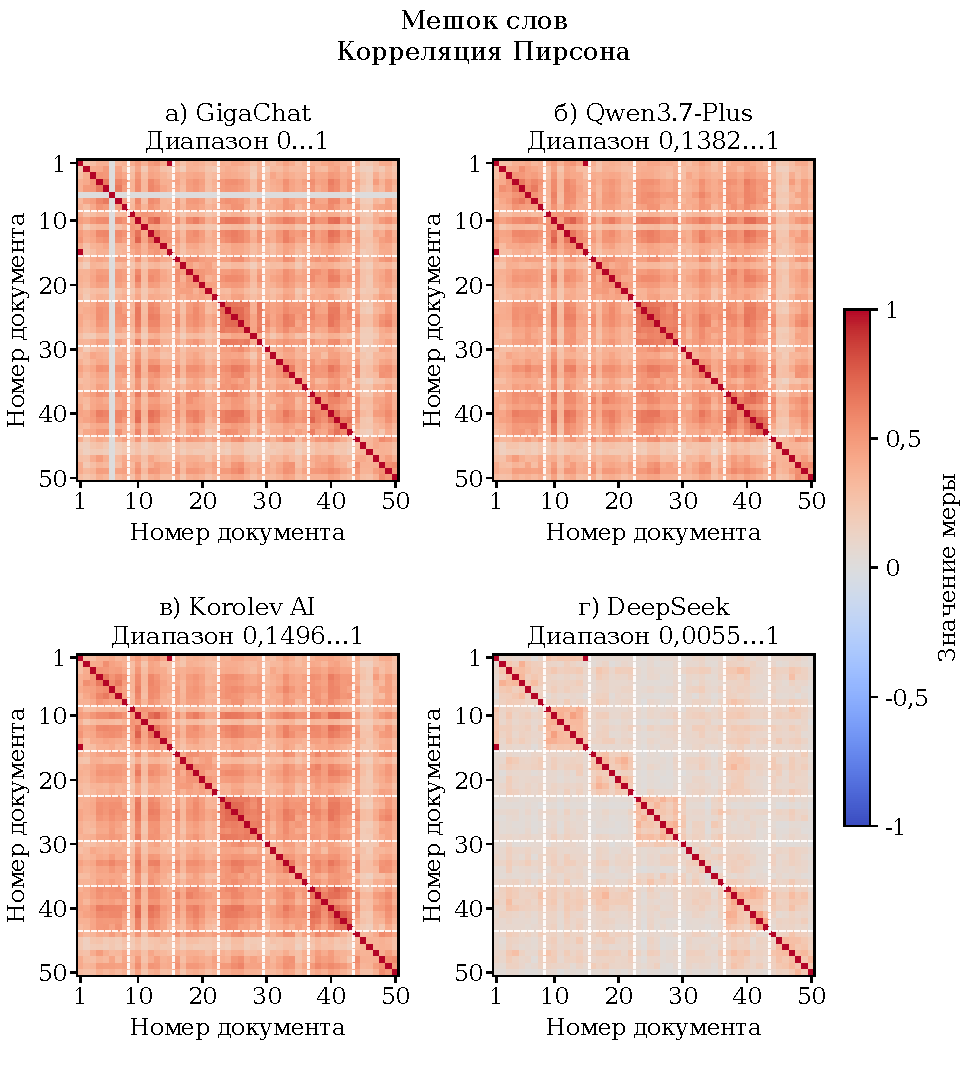
\includegraphics[width=\linewidth,height=0.78\textheight,keepaspectratio]{comparison_count_bow_pearson.pdf}
\caption{Корреляция Пирсона для представления мешка слов}
\label{fig:all-count-bow-pearson}
\end{figure}
\clearpage

Матрицы корреляции Спирмена для данного представления приведены на рисунке~\ref{fig:all-count-bow-spearman}.

\begin{figure}[H]
\centering
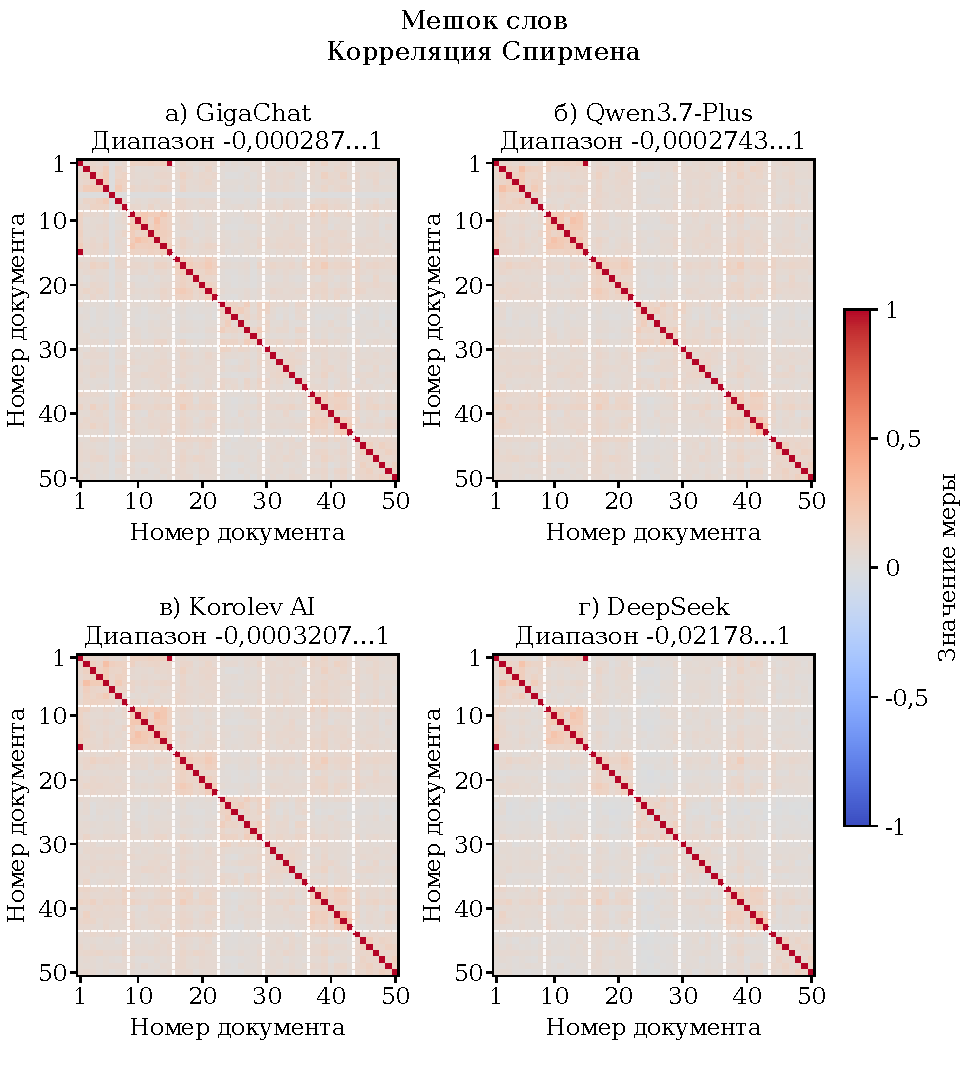
\includegraphics[width=\linewidth,height=0.78\textheight,keepaspectratio]{comparison_count_bow_spearman.pdf}
\caption{Корреляция Спирмена для представления мешка слов}
\label{fig:all-count-bow-spearman}
\end{figure}
\clearpage

Матрицы взвешенного коэффициента Жаккара для данного представления приведены на рисунке~\ref{fig:all-count-bow-weighted-jaccard}.

\begin{figure}[H]
\centering
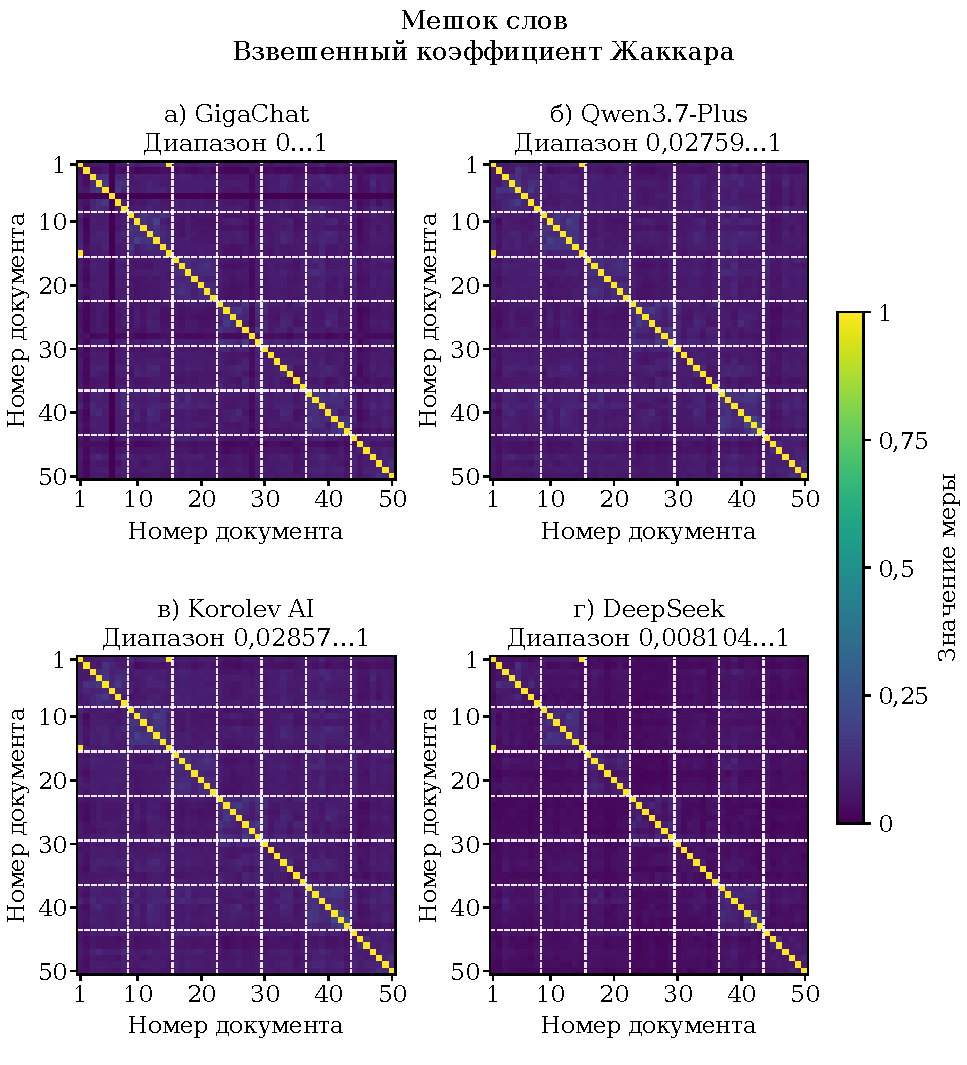
\includegraphics[width=\linewidth,height=0.78\textheight,keepaspectratio]{comparison_count_bow_weighted_jaccard.pdf}
\caption{Взвешенный коэффициент Жаккара для представления мешка слов}
\label{fig:all-count-bow-weighted-jaccard}
\end{figure}
\clearpage

Матрицы взвешенного коэффициента Дайса для данного представления приведены на рисунке~\ref{fig:all-count-bow-weighted-dice}.

\begin{figure}[H]
\centering
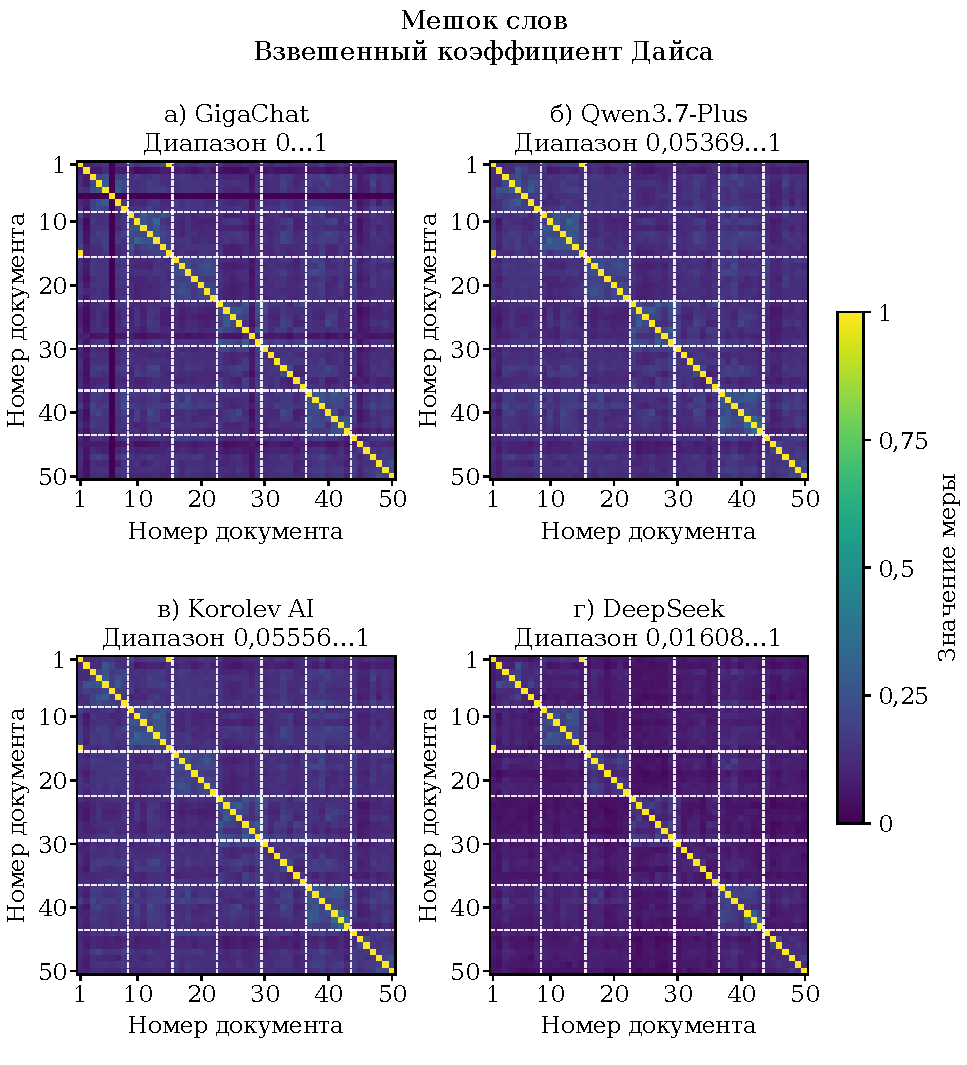
\includegraphics[width=\linewidth,height=0.78\textheight,keepaspectratio]{comparison_count_bow_weighted_dice.pdf}
\caption{Взвешенный коэффициент Дайса для представления мешка слов}
\label{fig:all-count-bow-weighted-dice}
\end{figure}
\clearpage

Матрицы евклидова расстояния для данного представления приведены на рисунке~\ref{fig:all-count-bow-euclidean}.

\begin{figure}[H]
\centering
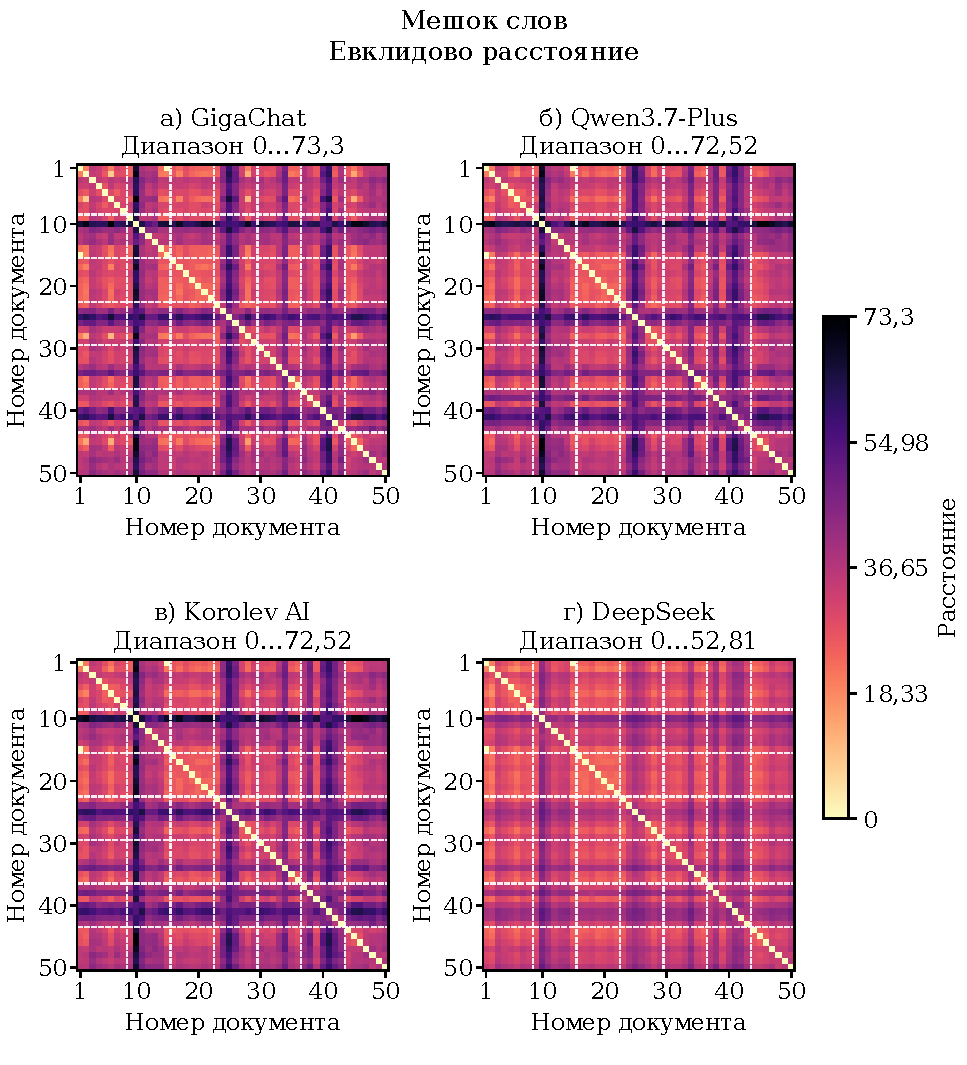
\includegraphics[width=\linewidth,height=0.78\textheight,keepaspectratio]{comparison_count_bow_euclidean.pdf}
\caption{Евклидово расстояние для представления мешка слов}
\label{fig:all-count-bow-euclidean}
\end{figure}
\clearpage

Матрицы манхэттенского расстояния для данного представления приведены на рисунке~\ref{fig:all-count-bow-manhattan}.

\begin{figure}[H]
\centering
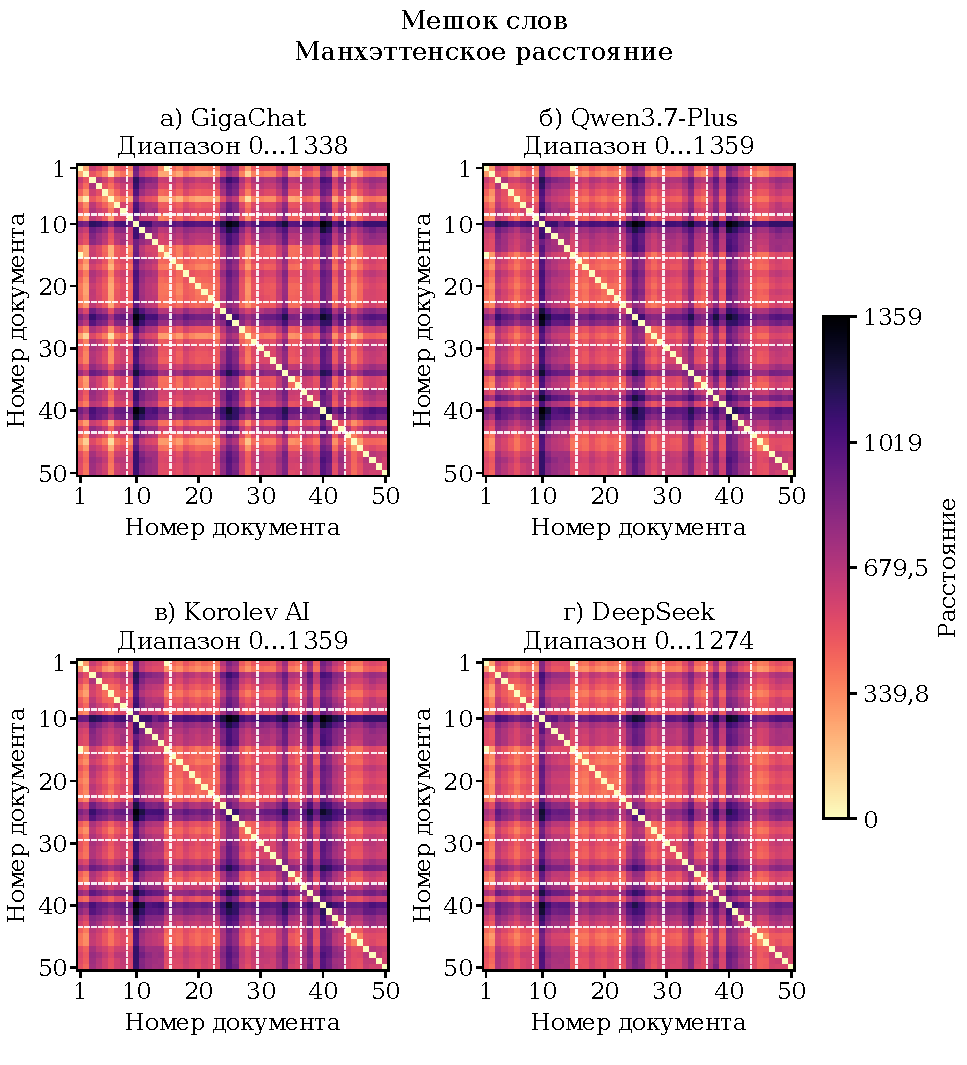
\includegraphics[width=\linewidth,height=0.78\textheight,keepaspectratio]{comparison_count_bow_manhattan.pdf}
\caption{Манхэттенское расстояние для представления мешка слов}
\label{fig:all-count-bow-manhattan}
\end{figure}
\clearpage

Матрицы чебышёвского расстояния для данного представления приведены на рисунке~\ref{fig:all-count-bow-chebyshev}.

\begin{figure}[H]
\centering
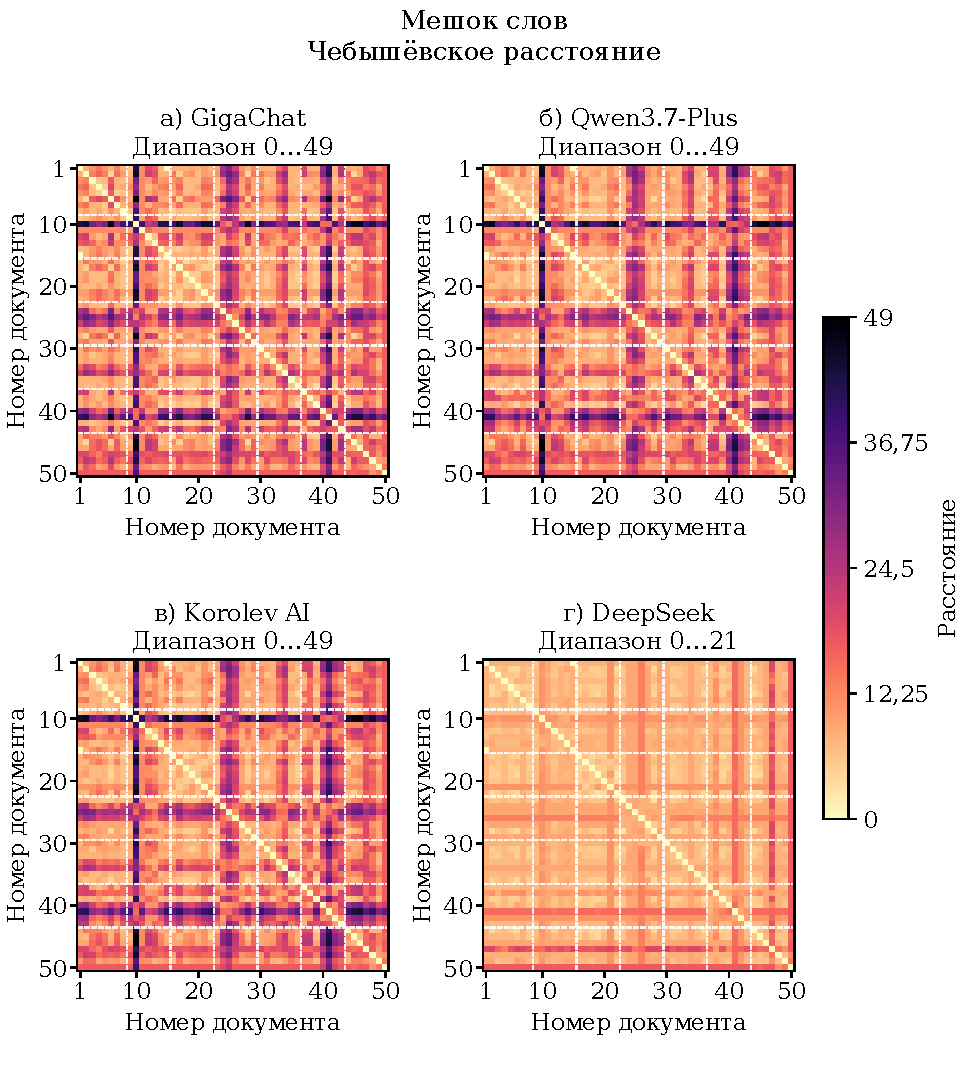
\includegraphics[width=\linewidth,height=0.78\textheight,keepaspectratio]{comparison_count_bow_chebyshev.pdf}
\caption{Чебышёвское расстояние для представления мешка слов}
\label{fig:all-count-bow-chebyshev}
\end{figure}
\clearpage

Матрицы близости по евклидову расстоянию для данного представления приведены на рисунке~\ref{fig:all-count-bow-euclidean-closeness}.

\begin{figure}[H]
\centering
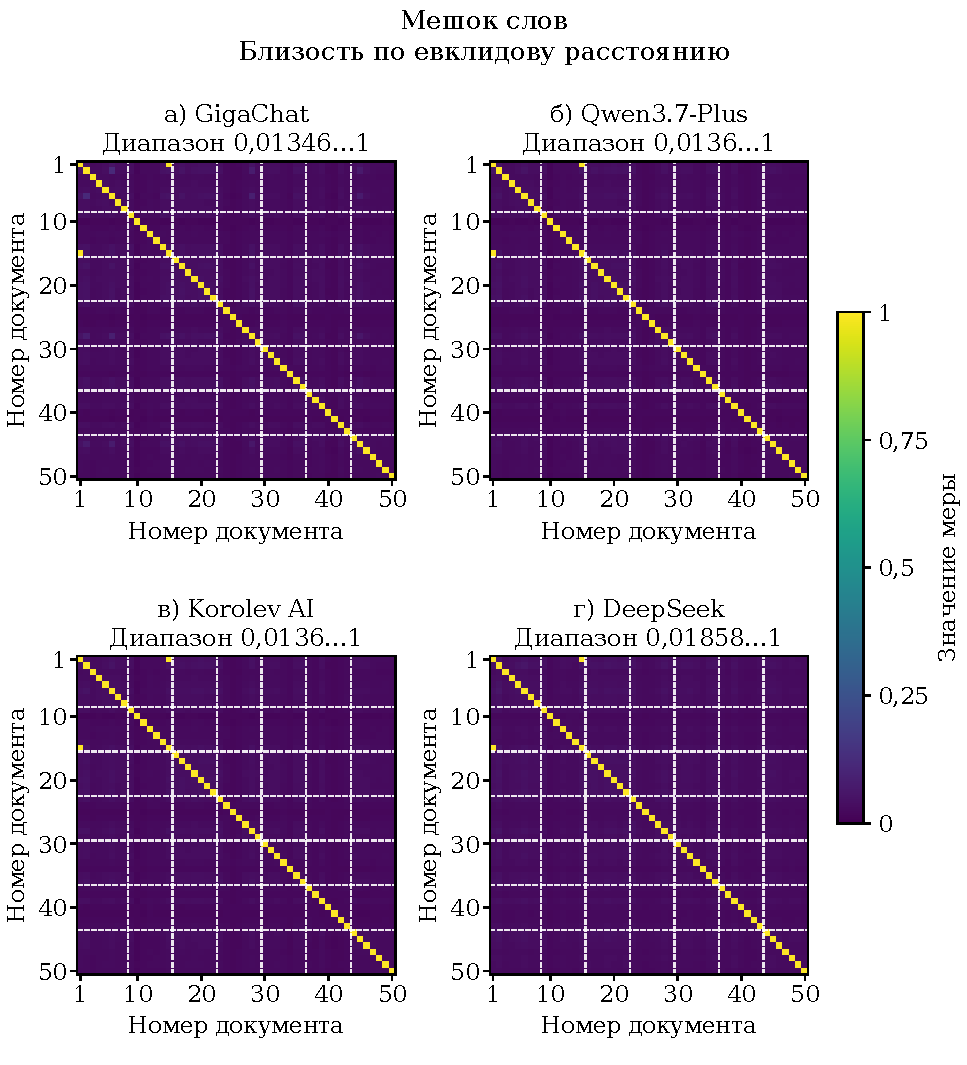
\includegraphics[width=\linewidth,height=0.78\textheight,keepaspectratio]{comparison_count_bow_euclidean_closeness.pdf}
\caption{Близость по евклидову расстоянию для представления мешка слов}
\label{fig:all-count-bow-euclidean-closeness}
\end{figure}
\clearpage

Матрицы близости по манхэттенскому расстоянию для данного представления приведены на рисунке~\ref{fig:all-count-bow-manhattan-closeness}.

\begin{figure}[H]
\centering
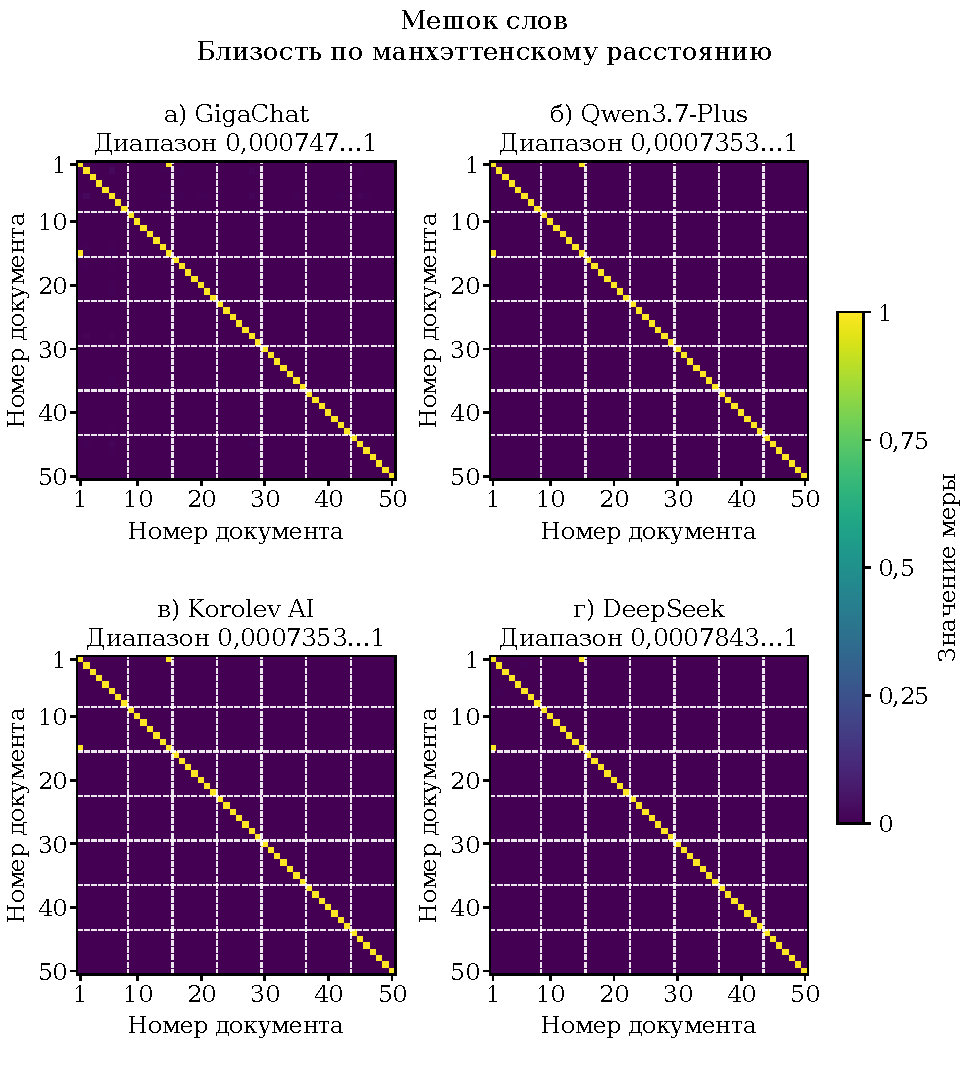
\includegraphics[width=\linewidth,height=0.78\textheight,keepaspectratio]{comparison_count_bow_manhattan_closeness.pdf}
\caption{Близость по манхэттенскому расстоянию для представления мешка слов}
\label{fig:all-count-bow-manhattan-closeness}
\end{figure}
\clearpage

Матрицы близости по чебышёвскому расстоянию для данного представления приведены на рисунке~\ref{fig:all-count-bow-chebyshev-closeness}.

\begin{figure}[H]
\centering
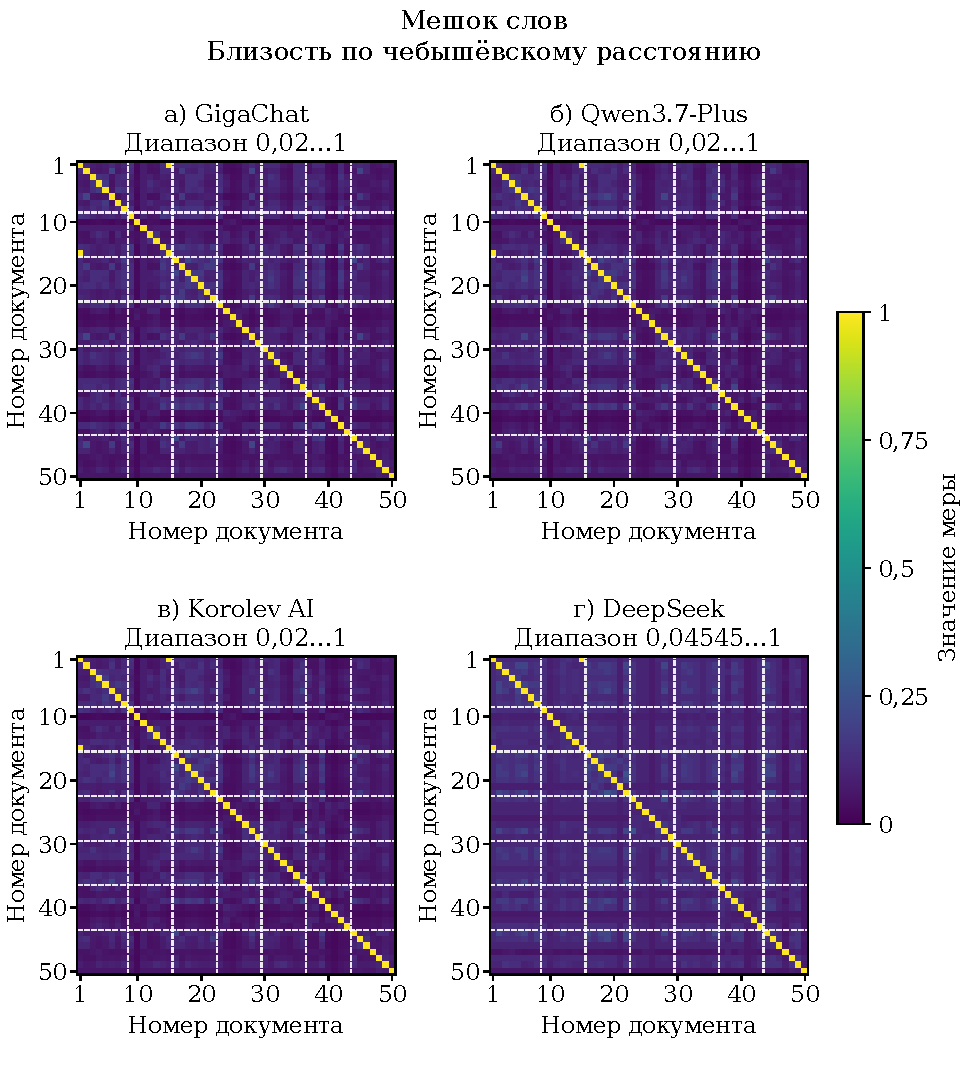
\includegraphics[width=\linewidth,height=0.78\textheight,keepaspectratio]{comparison_count_bow_chebyshev_closeness.pdf}
\caption{Близость по чебышёвскому расстоянию для представления мешка слов}
\label{fig:all-count-bow-chebyshev-closeness}
\end{figure}
\clearpage

\clearpage
\subsection{Представление TF--IDF по леммам}

Матрицы косинусной близости для данного представления приведены на рисунке~\ref{fig:all-tfidf-lemma-cosine}.

\begin{figure}[H]
\centering
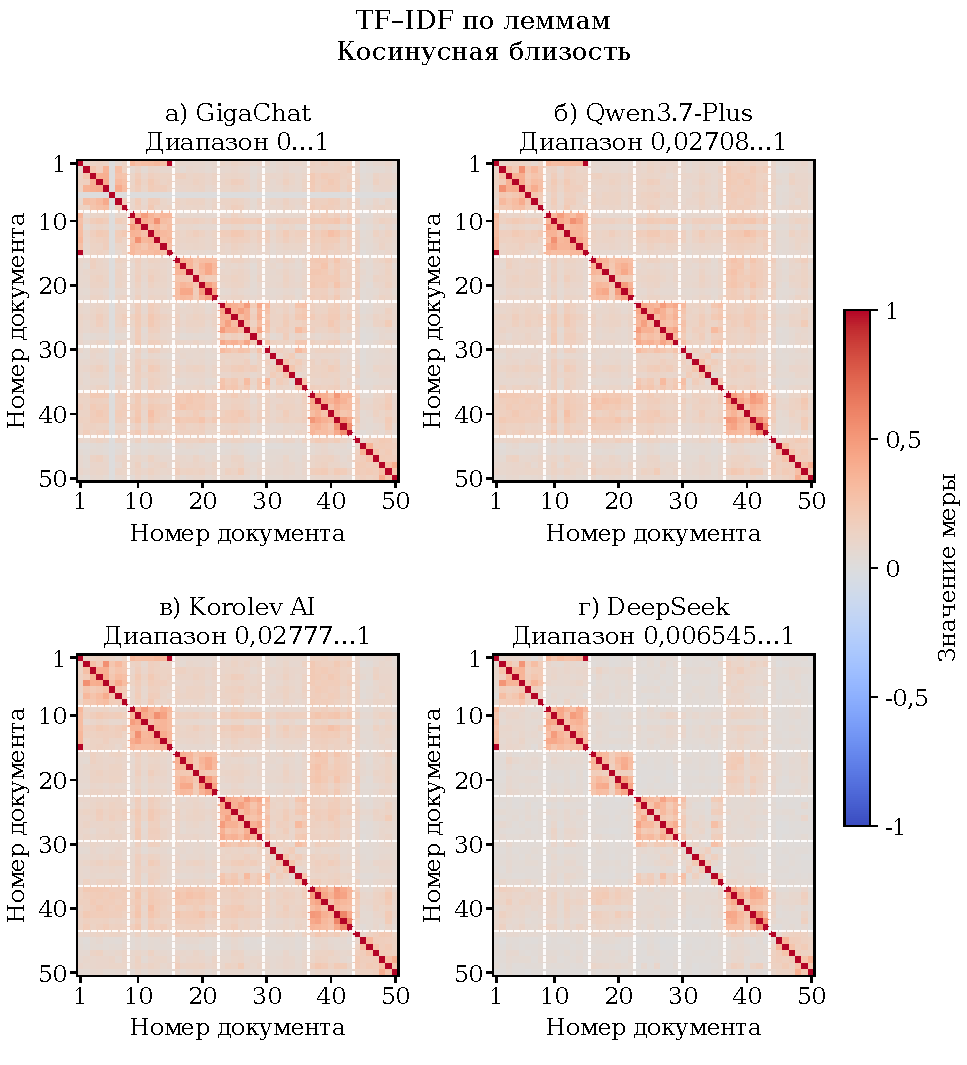
\includegraphics[width=\linewidth,height=0.78\textheight,keepaspectratio]{comparison_tfidf_lemma_cosine.pdf}
\caption{Косинусная близость для представления TF--IDF по леммам}
\label{fig:all-tfidf-lemma-cosine}
\end{figure}
\clearpage

Матрицы корреляции Пирсона для данного представления приведены на рисунке~\ref{fig:all-tfidf-lemma-pearson}.

\begin{figure}[H]
\centering
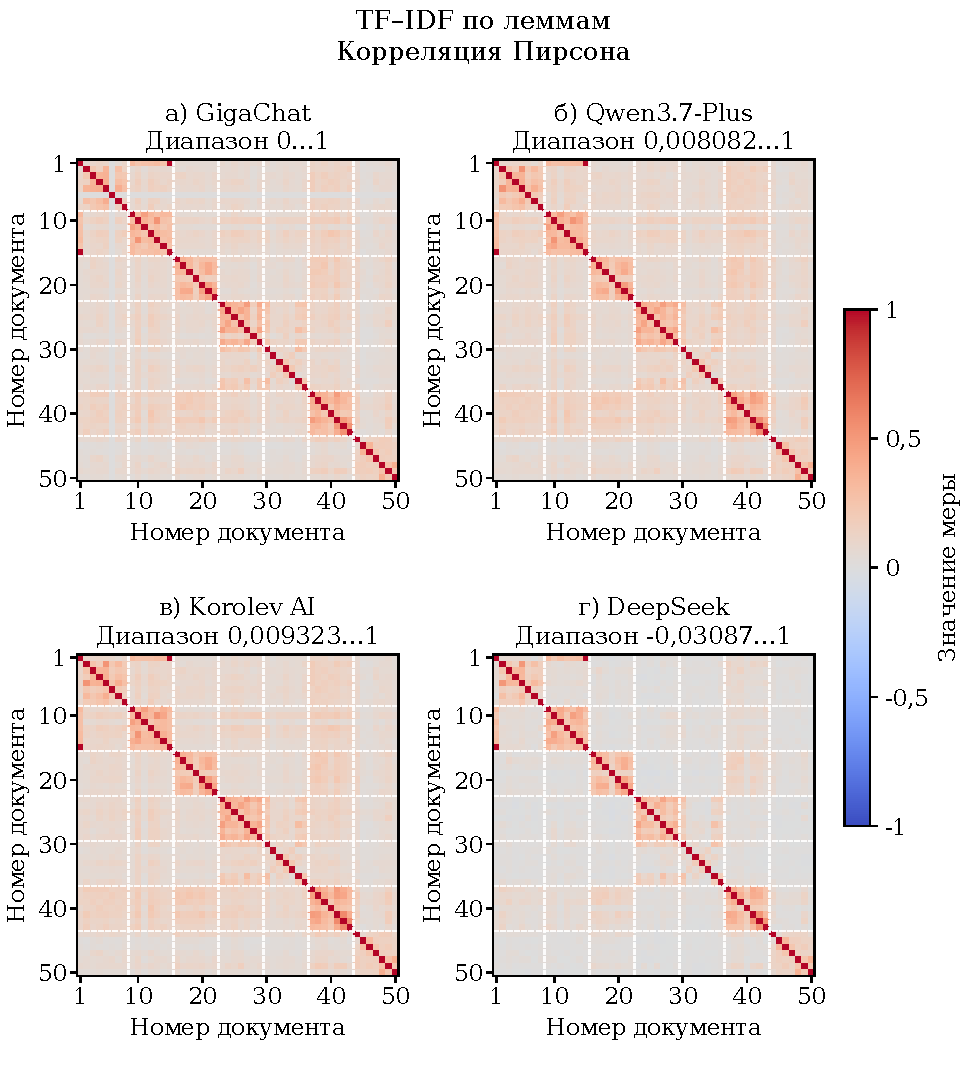
\includegraphics[width=\linewidth,height=0.78\textheight,keepaspectratio]{comparison_tfidf_lemma_pearson.pdf}
\caption{Корреляция Пирсона для представления TF--IDF по леммам}
\label{fig:all-tfidf-lemma-pearson}
\end{figure}
\clearpage

Матрицы корреляции Спирмена для данного представления приведены на рисунке~\ref{fig:all-tfidf-lemma-spearman}.

\begin{figure}[H]
\centering
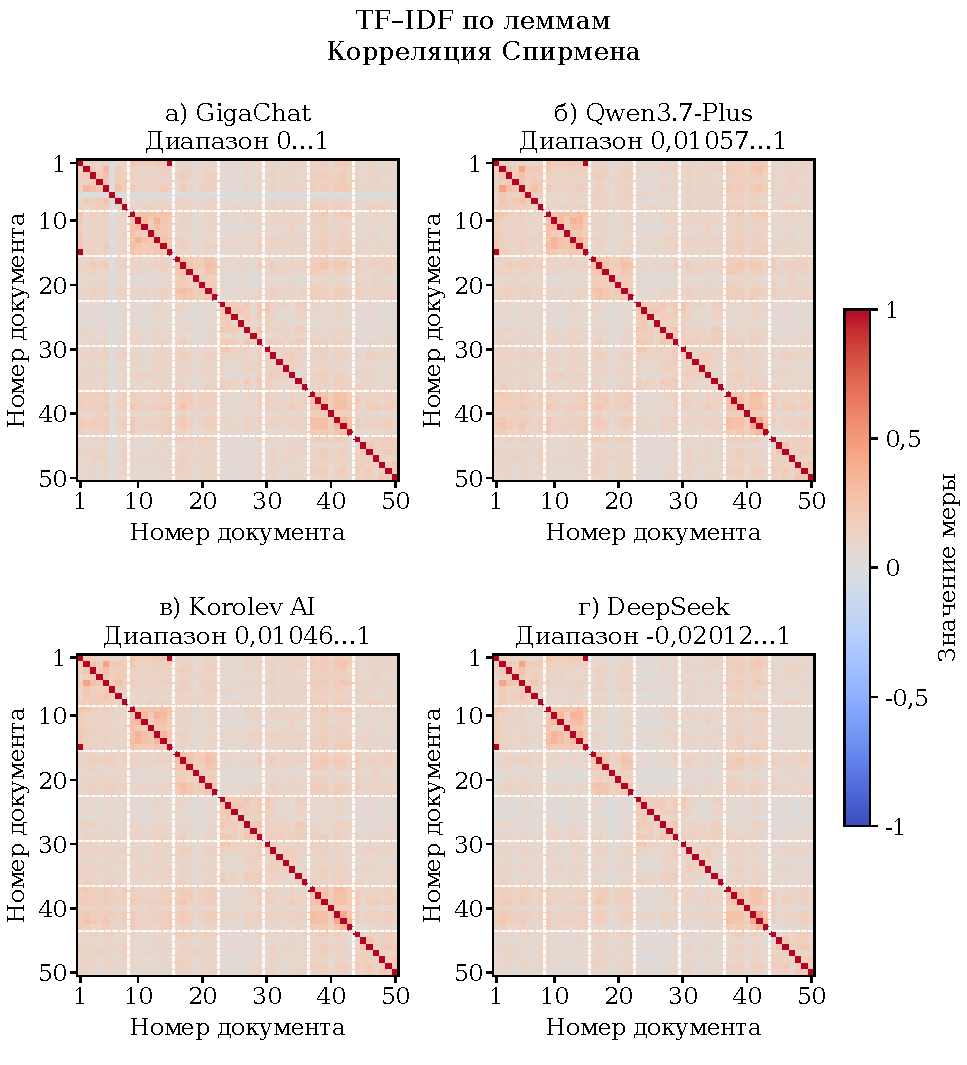
\includegraphics[width=\linewidth,height=0.78\textheight,keepaspectratio]{comparison_tfidf_lemma_spearman.pdf}
\caption{Корреляция Спирмена для представления TF--IDF по леммам}
\label{fig:all-tfidf-lemma-spearman}
\end{figure}
\clearpage

Матрицы взвешенного коэффициента Жаккара для данного представления приведены на рисунке~\ref{fig:all-tfidf-lemma-weighted-jaccard}.

\begin{figure}[H]
\centering
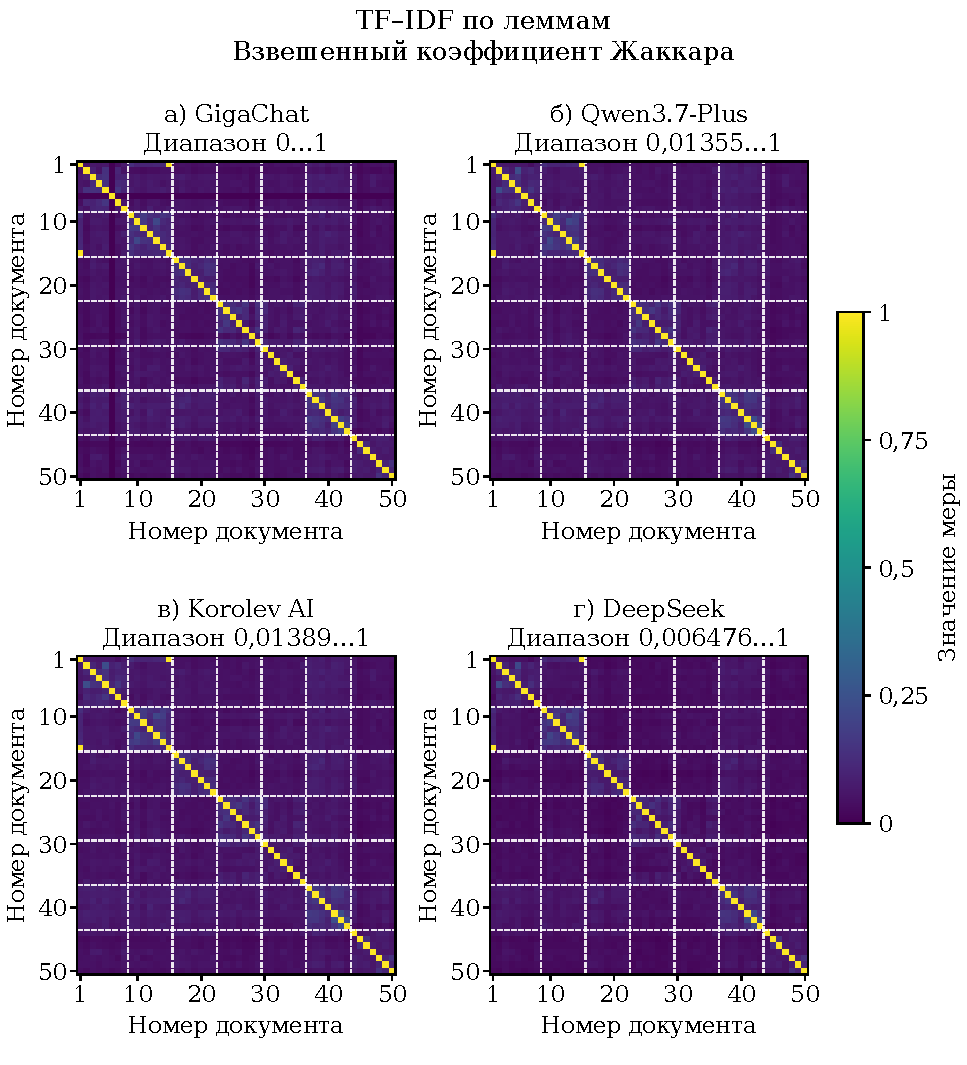
\includegraphics[width=\linewidth,height=0.78\textheight,keepaspectratio]{comparison_tfidf_lemma_weighted_jaccard.pdf}
\caption{Взвешенный коэффициент Жаккара для представления TF--IDF по леммам}
\label{fig:all-tfidf-lemma-weighted-jaccard}
\end{figure}
\clearpage

Матрицы взвешенного коэффициента Дайса для данного представления приведены на рисунке~\ref{fig:all-tfidf-lemma-weighted-dice}.

\begin{figure}[H]
\centering
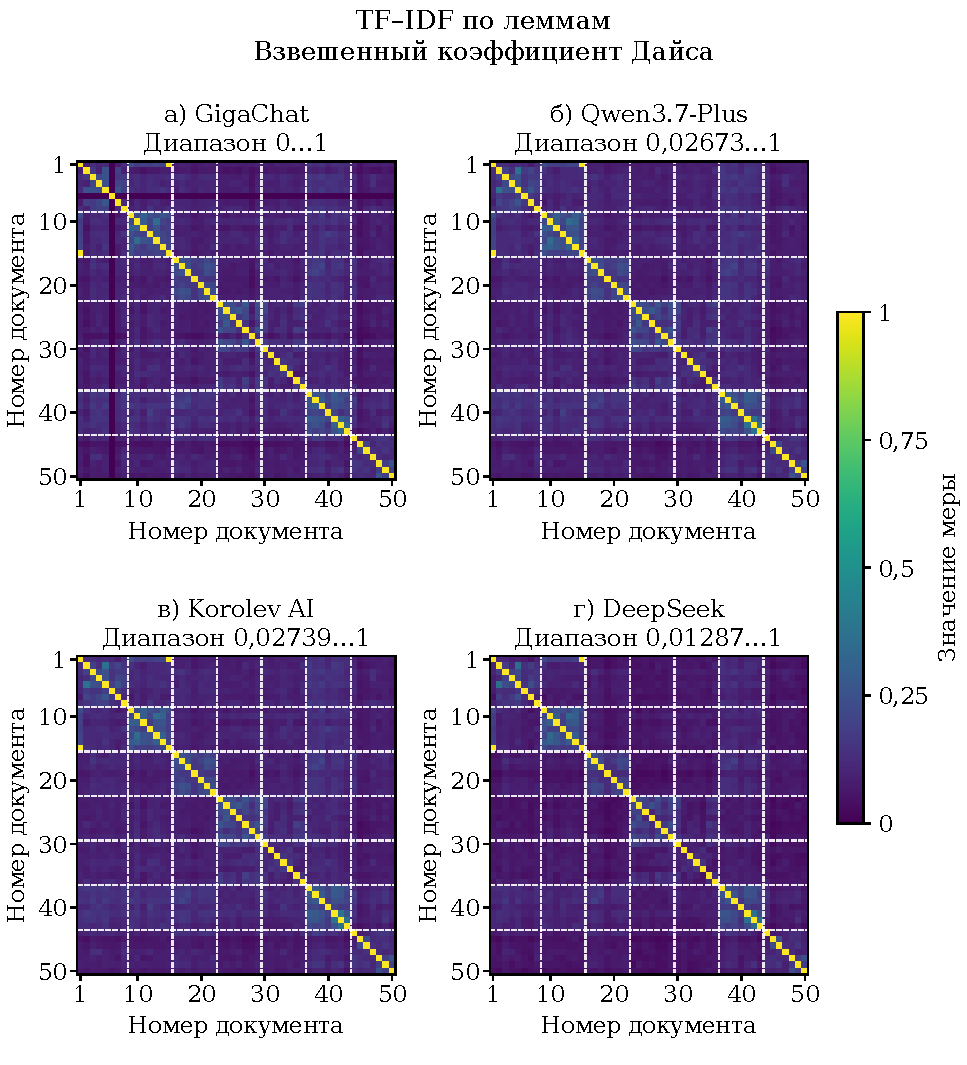
\includegraphics[width=\linewidth,height=0.78\textheight,keepaspectratio]{comparison_tfidf_lemma_weighted_dice.pdf}
\caption{Взвешенный коэффициент Дайса для представления TF--IDF по леммам}
\label{fig:all-tfidf-lemma-weighted-dice}
\end{figure}
\clearpage

Матрицы евклидова расстояния для данного представления приведены на рисунке~\ref{fig:all-tfidf-lemma-euclidean}.

\begin{figure}[H]
\centering
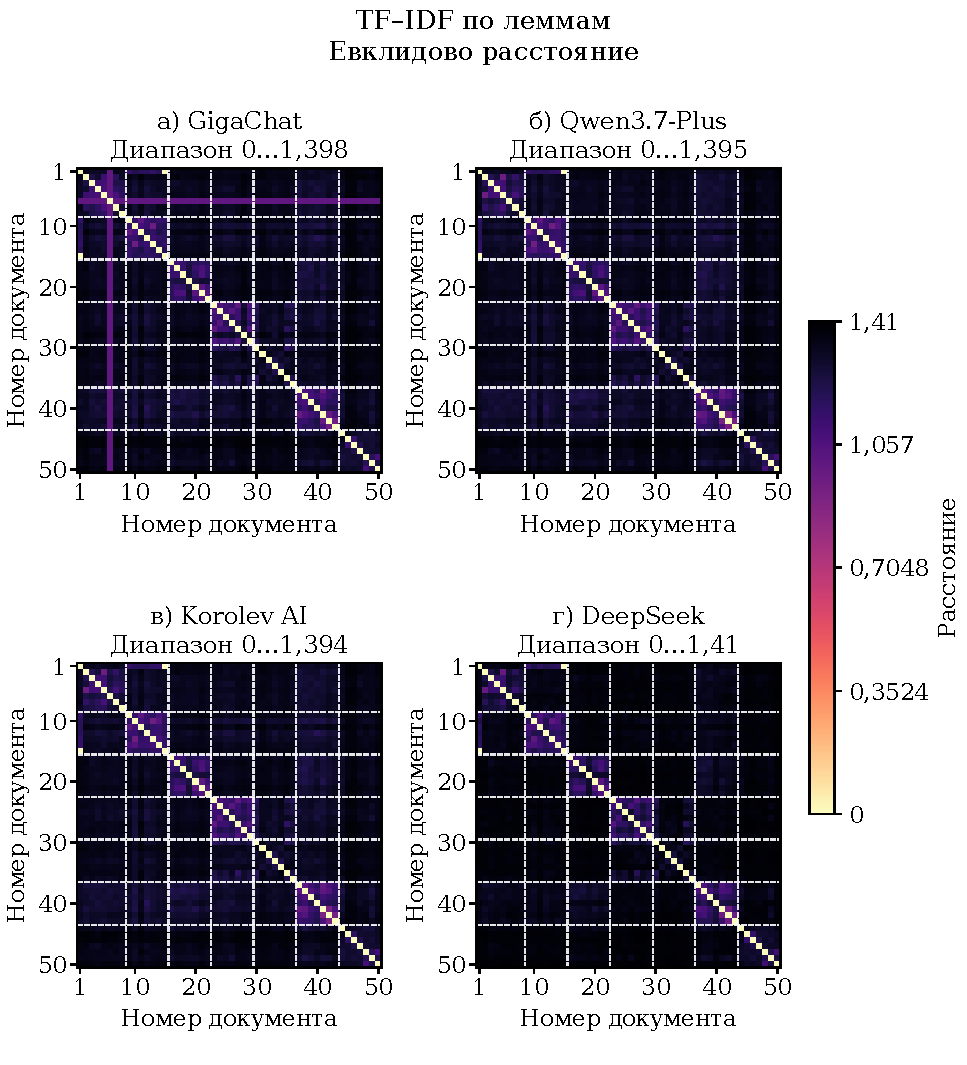
\includegraphics[width=\linewidth,height=0.78\textheight,keepaspectratio]{comparison_tfidf_lemma_euclidean.pdf}
\caption{Евклидово расстояние для представления TF--IDF по леммам}
\label{fig:all-tfidf-lemma-euclidean}
\end{figure}
\clearpage

Матрицы манхэттенского расстояния для данного представления приведены на рисунке~\ref{fig:all-tfidf-lemma-manhattan}.

\begin{figure}[H]
\centering
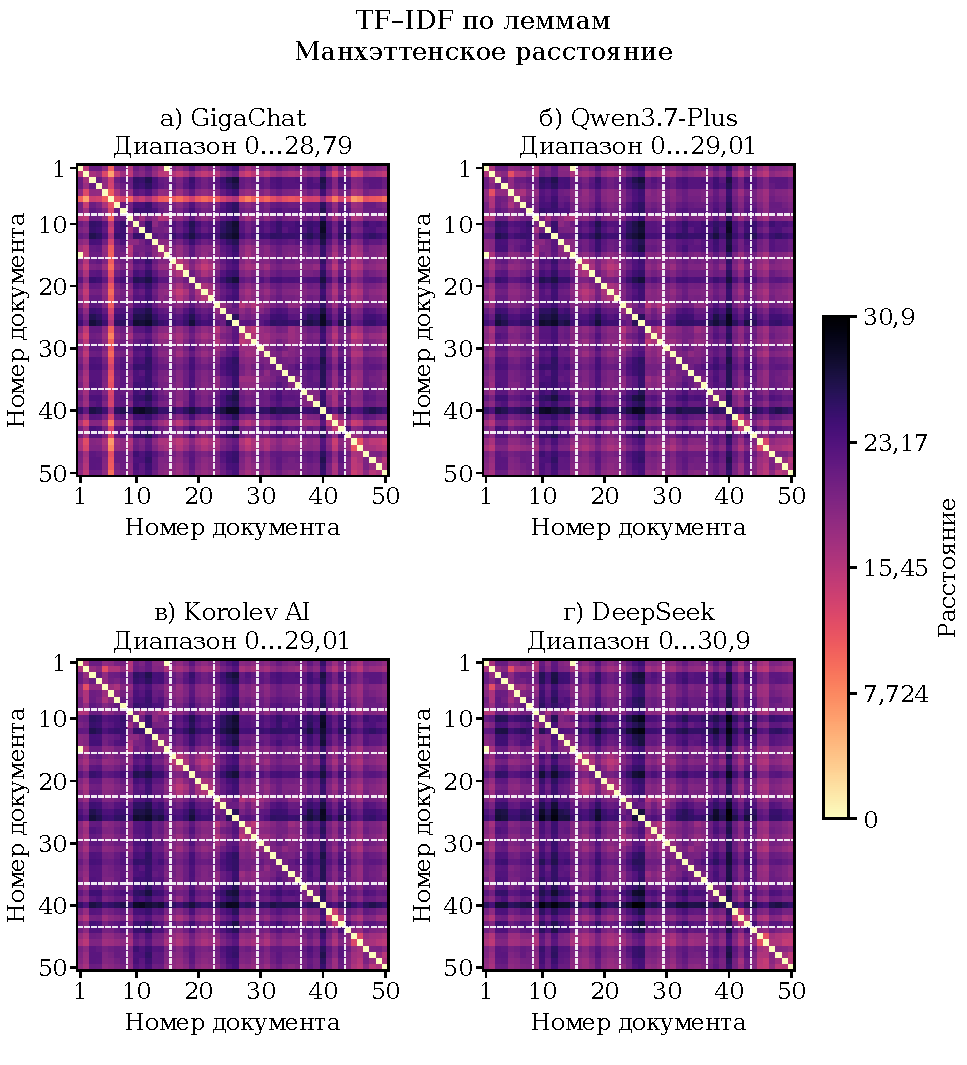
\includegraphics[width=\linewidth,height=0.78\textheight,keepaspectratio]{comparison_tfidf_lemma_manhattan.pdf}
\caption{Манхэттенское расстояние для представления TF--IDF по леммам}
\label{fig:all-tfidf-lemma-manhattan}
\end{figure}
\clearpage

Матрицы чебышёвского расстояния для данного представления приведены на рисунке~\ref{fig:all-tfidf-lemma-chebyshev}.

\begin{figure}[H]
\centering
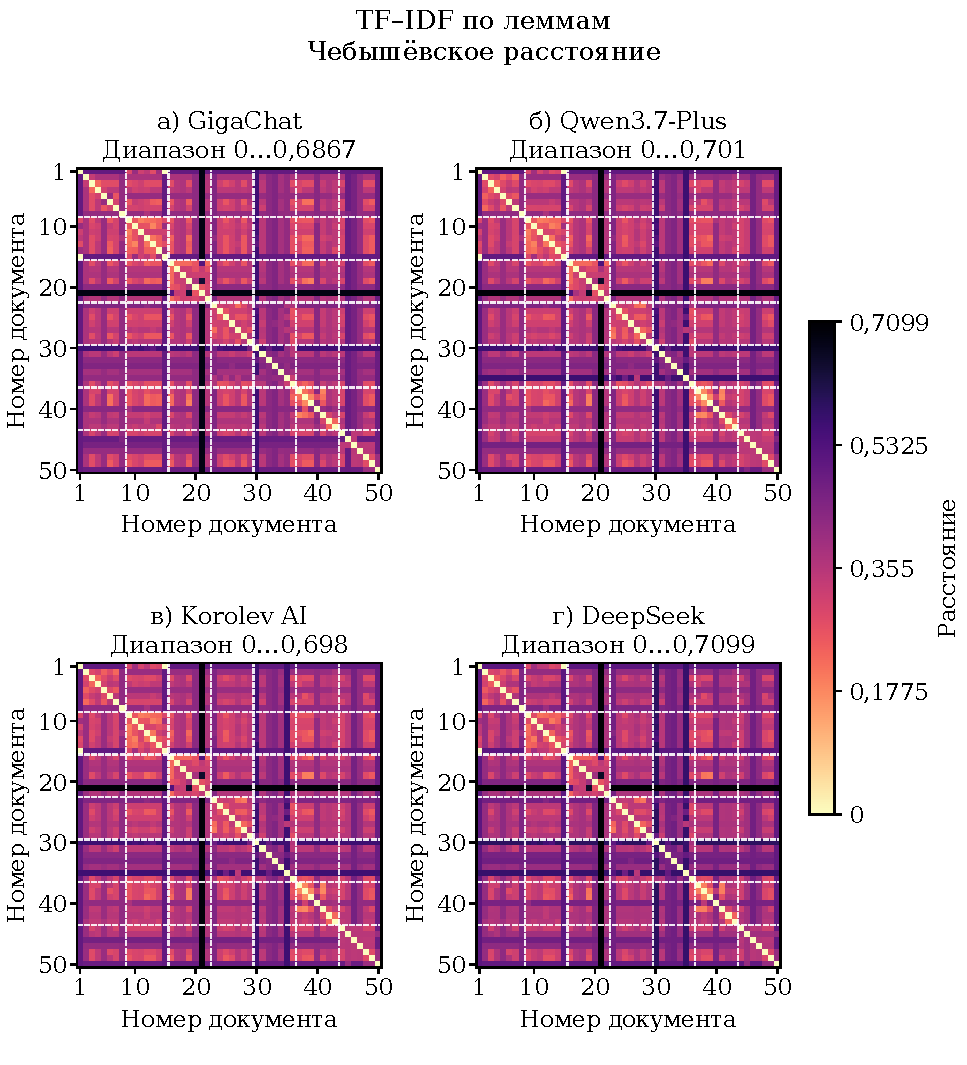
\includegraphics[width=\linewidth,height=0.78\textheight,keepaspectratio]{comparison_tfidf_lemma_chebyshev.pdf}
\caption{Чебышёвское расстояние для представления TF--IDF по леммам}
\label{fig:all-tfidf-lemma-chebyshev}
\end{figure}
\clearpage

Матрицы близости по евклидову расстоянию для данного представления приведены на рисунке~\ref{fig:all-tfidf-lemma-euclidean-closeness}.

\begin{figure}[H]
\centering
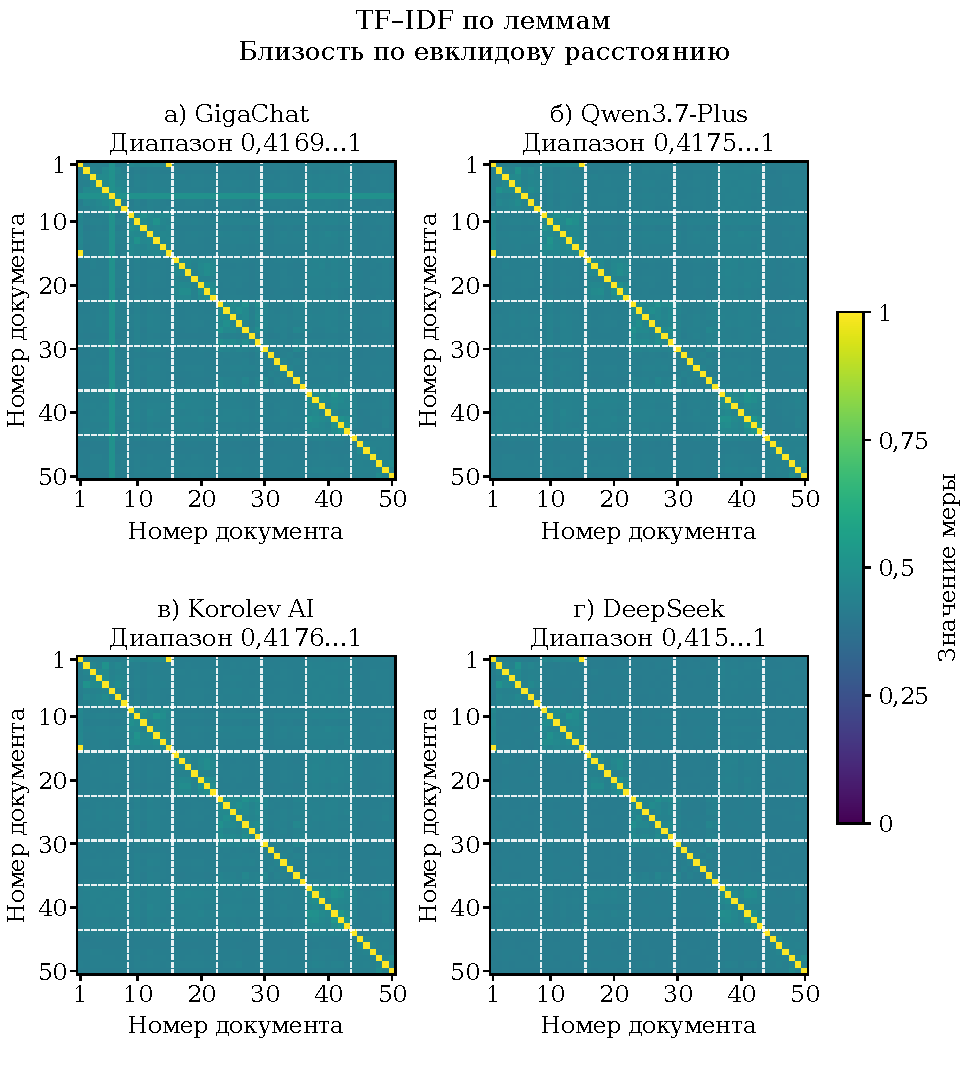
\includegraphics[width=\linewidth,height=0.78\textheight,keepaspectratio]{comparison_tfidf_lemma_euclidean_closeness.pdf}
\caption{Близость по евклидову расстоянию для представления TF--IDF по леммам}
\label{fig:all-tfidf-lemma-euclidean-closeness}
\end{figure}
\clearpage

Матрицы близости по манхэттенскому расстоянию для данного представления приведены на рисунке~\ref{fig:all-tfidf-lemma-manhattan-closeness}.

\begin{figure}[H]
\centering
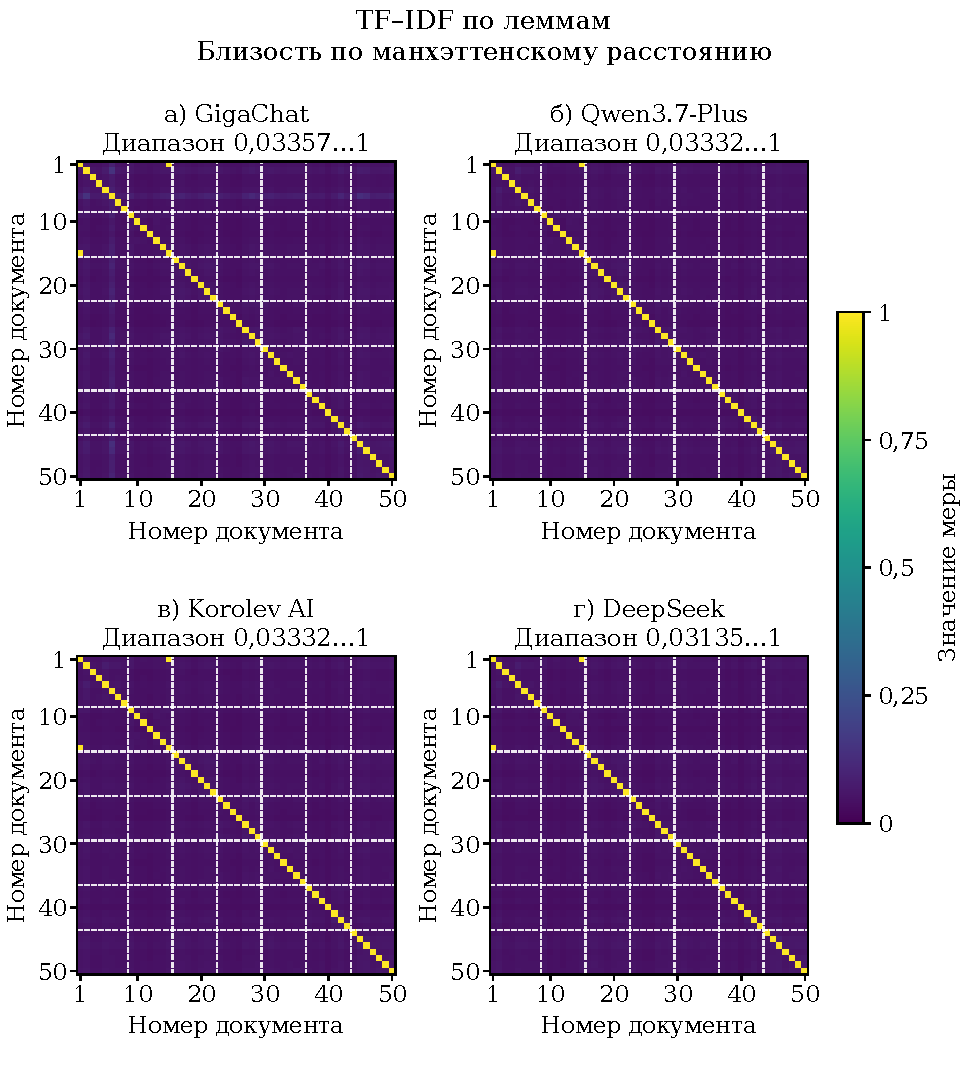
\includegraphics[width=\linewidth,height=0.78\textheight,keepaspectratio]{comparison_tfidf_lemma_manhattan_closeness.pdf}
\caption{Близость по манхэттенскому расстоянию для представления TF--IDF по леммам}
\label{fig:all-tfidf-lemma-manhattan-closeness}
\end{figure}
\clearpage

Матрицы близости по чебышёвскому расстоянию для данного представления приведены на рисунке~\ref{fig:all-tfidf-lemma-chebyshev-closeness}.

\begin{figure}[H]
\centering
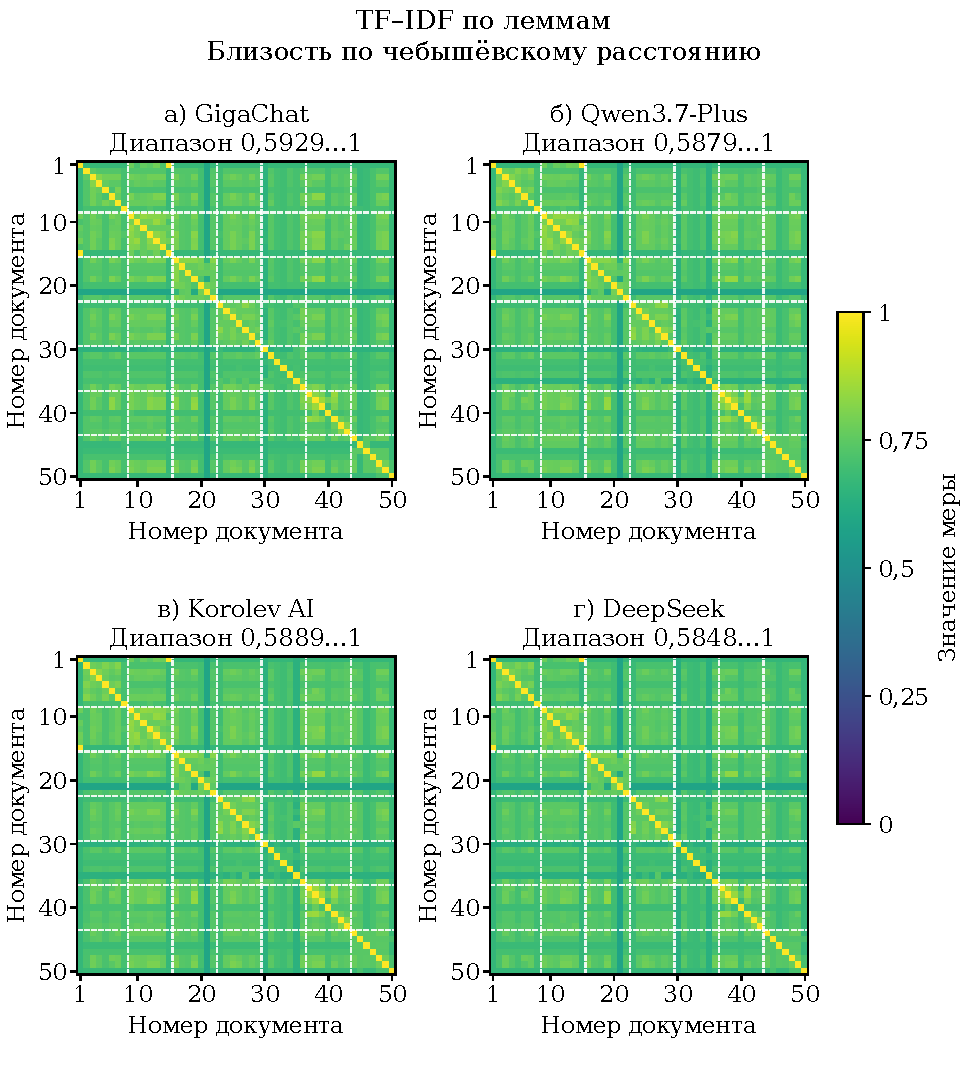
\includegraphics[width=\linewidth,height=0.78\textheight,keepaspectratio]{comparison_tfidf_lemma_chebyshev_closeness.pdf}
\caption{Близость по чебышёвскому расстоянию для представления TF--IDF по леммам}
\label{fig:all-tfidf-lemma-chebyshev-closeness}
\end{figure}
\clearpage

\clearpage
\subsection{Представление BGE-M3}

Матрицы косинусной близости для данного представления приведены на рисунке~\ref{fig:all-bge-m3-cosine}.

\begin{figure}[H]
\centering
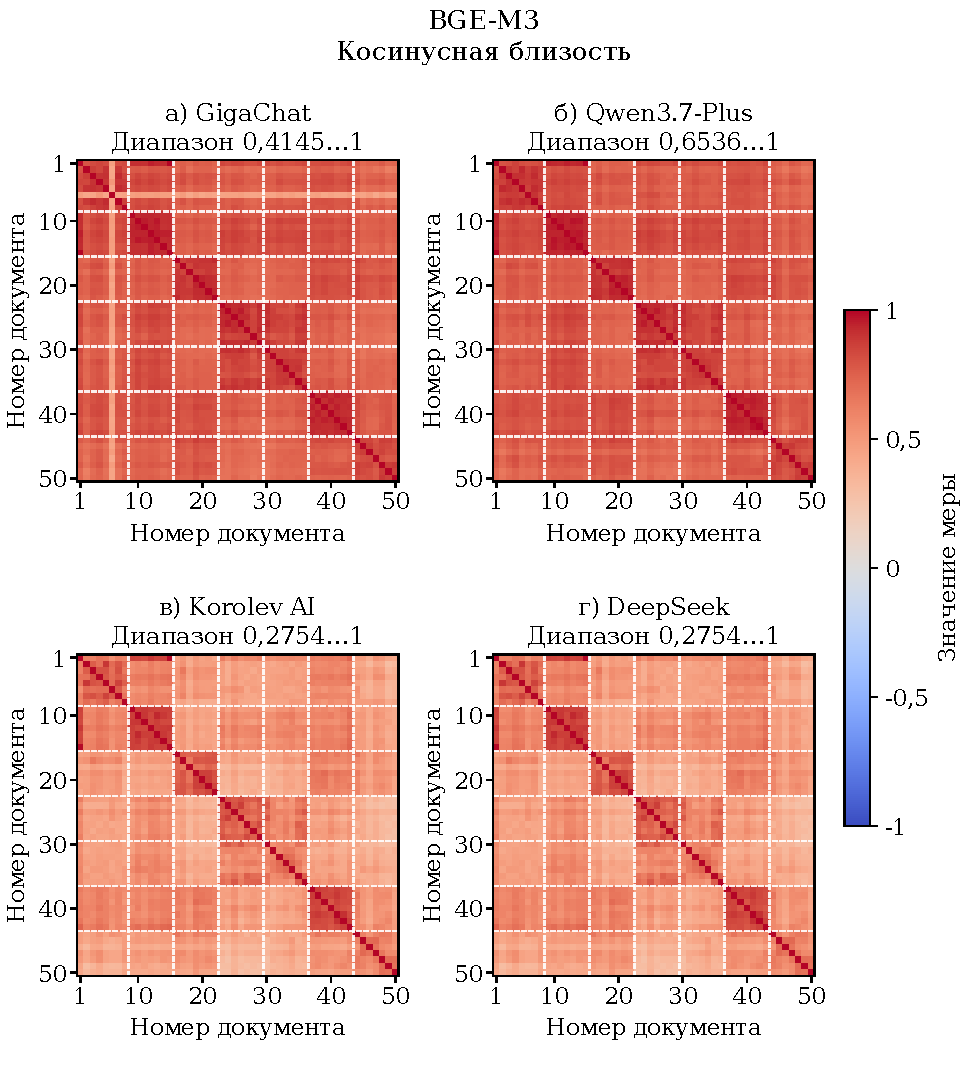
\includegraphics[width=\linewidth,height=0.78\textheight,keepaspectratio]{comparison_bge_m3_cosine.pdf}
\caption{Косинусная близость для представления BGE-M3}
\label{fig:all-bge-m3-cosine}
\end{figure}
\clearpage

Матрицы корреляции Пирсона для данного представления приведены на рисунке~\ref{fig:all-bge-m3-pearson}.

\begin{figure}[H]
\centering
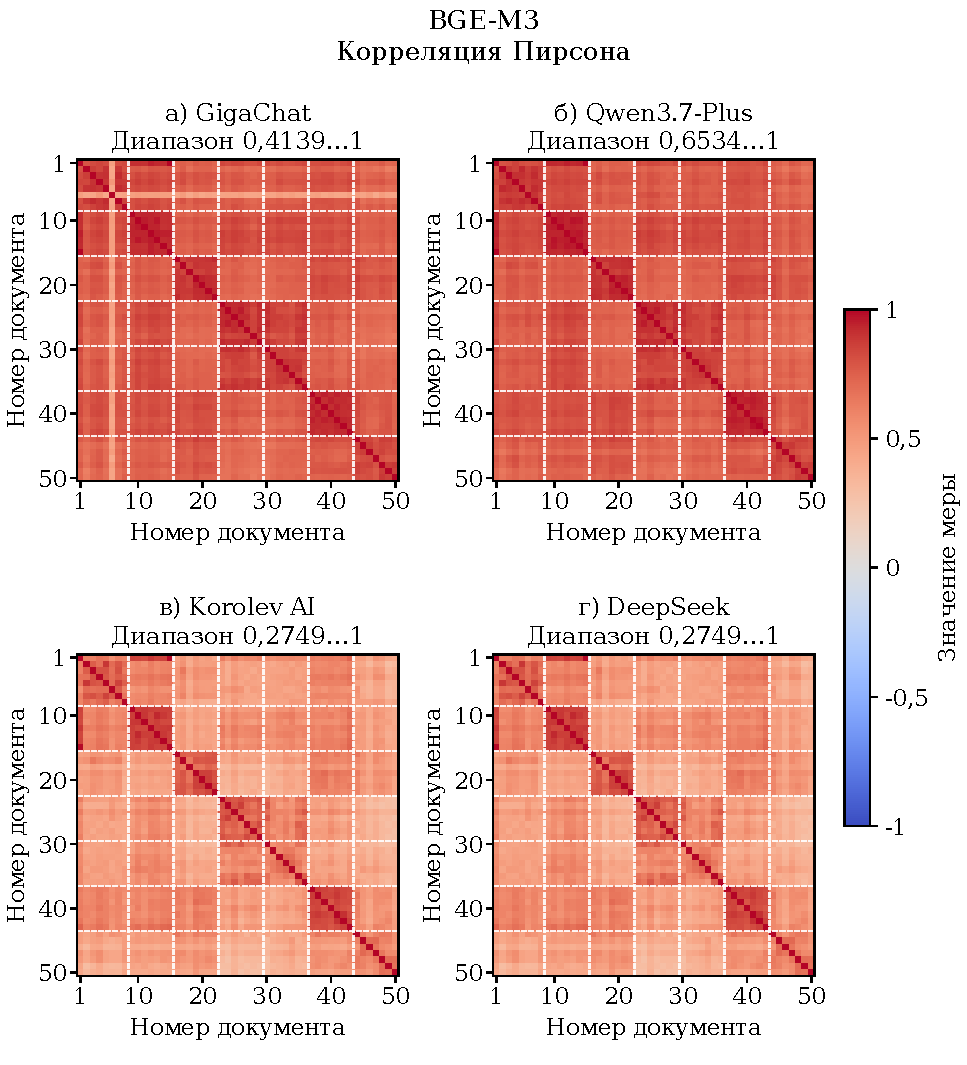
\includegraphics[width=\linewidth,height=0.78\textheight,keepaspectratio]{comparison_bge_m3_pearson.pdf}
\caption{Корреляция Пирсона для представления BGE-M3}
\label{fig:all-bge-m3-pearson}
\end{figure}
\clearpage

Матрицы корреляции Спирмена для данного представления приведены на рисунке~\ref{fig:all-bge-m3-spearman}.

\begin{figure}[H]
\centering
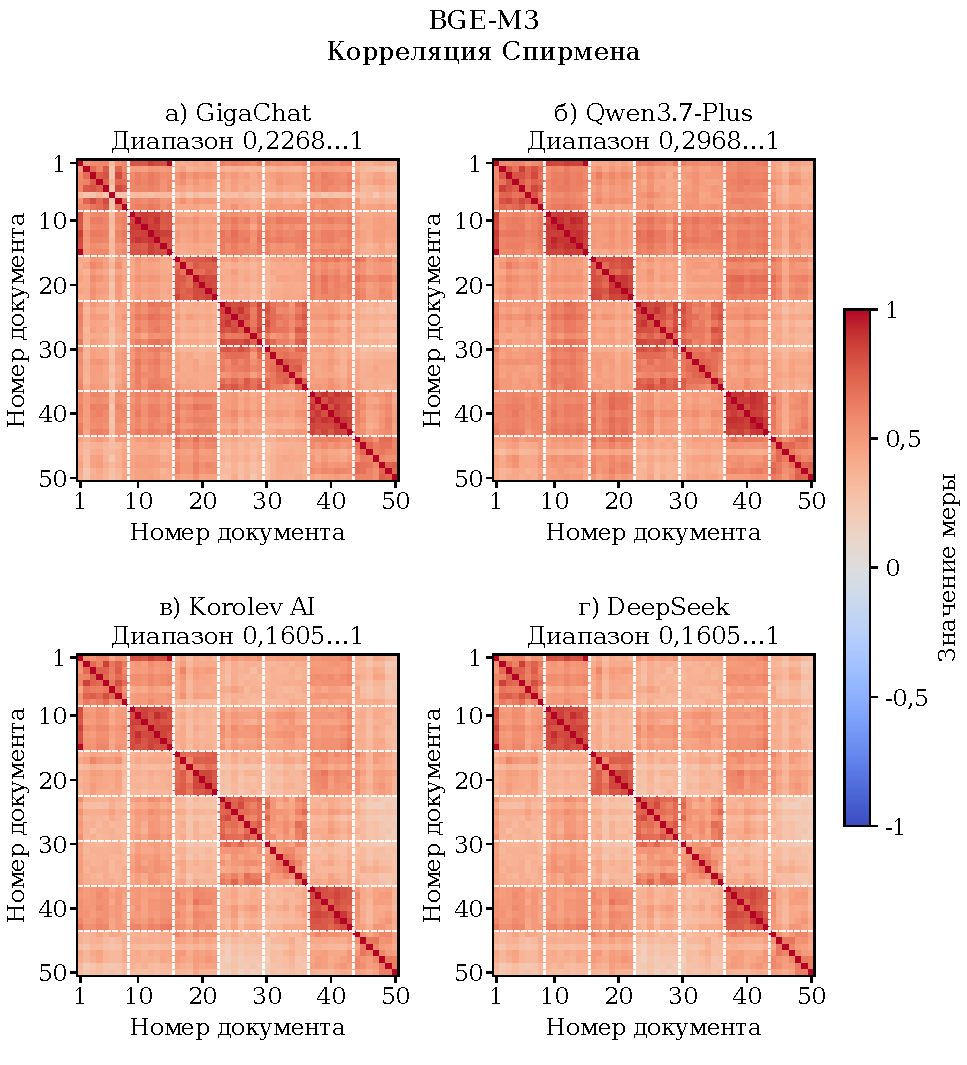
\includegraphics[width=\linewidth,height=0.78\textheight,keepaspectratio]{comparison_bge_m3_spearman.pdf}
\caption{Корреляция Спирмена для представления BGE-M3}
\label{fig:all-bge-m3-spearman}
\end{figure}
\clearpage

Матрицы взвешенного коэффициента Жаккара для данного представления приведены на рисунке~\ref{fig:all-bge-m3-weighted-jaccard}.

\begin{figure}[H]
\centering
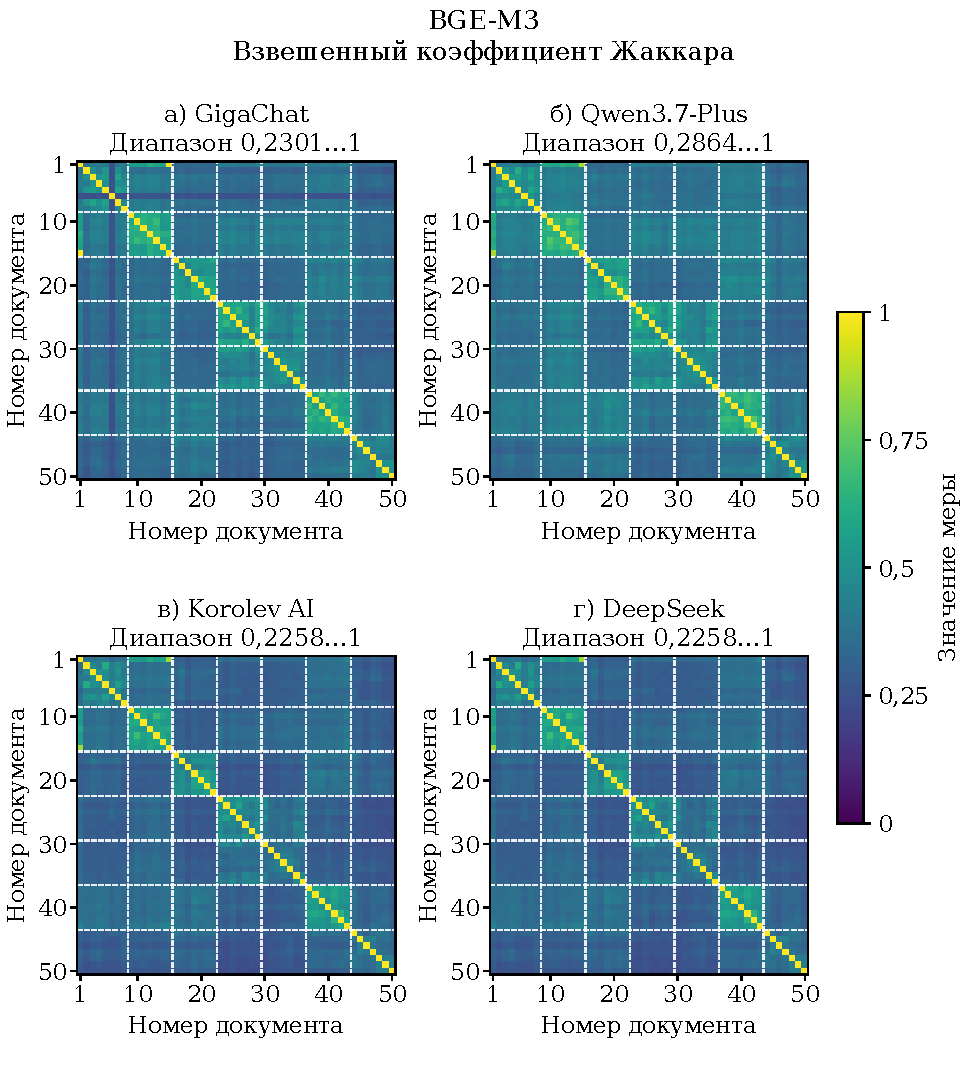
\includegraphics[width=\linewidth,height=0.78\textheight,keepaspectratio]{comparison_bge_m3_weighted_jaccard.pdf}
\caption{Взвешенный коэффициент Жаккара для представления BGE-M3}
\label{fig:all-bge-m3-weighted-jaccard}
\end{figure}
\clearpage

Матрицы взвешенного коэффициента Дайса для данного представления приведены на рисунке~\ref{fig:all-bge-m3-weighted-dice}.

\begin{figure}[H]
\centering
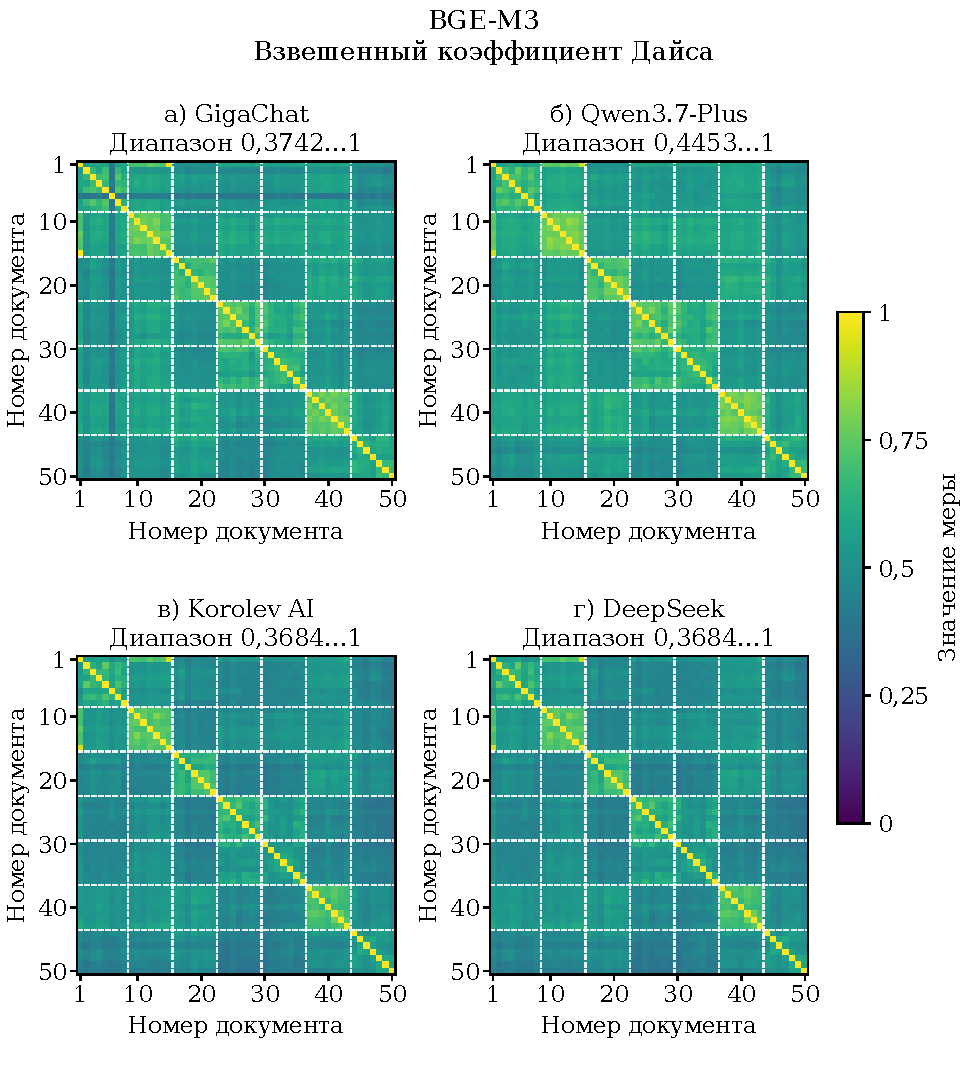
\includegraphics[width=\linewidth,height=0.78\textheight,keepaspectratio]{comparison_bge_m3_weighted_dice.pdf}
\caption{Взвешенный коэффициент Дайса для представления BGE-M3}
\label{fig:all-bge-m3-weighted-dice}
\end{figure}
\clearpage

Матрицы евклидова расстояния для данного представления приведены на рисунке~\ref{fig:all-bge-m3-euclidean}.

\begin{figure}[H]
\centering
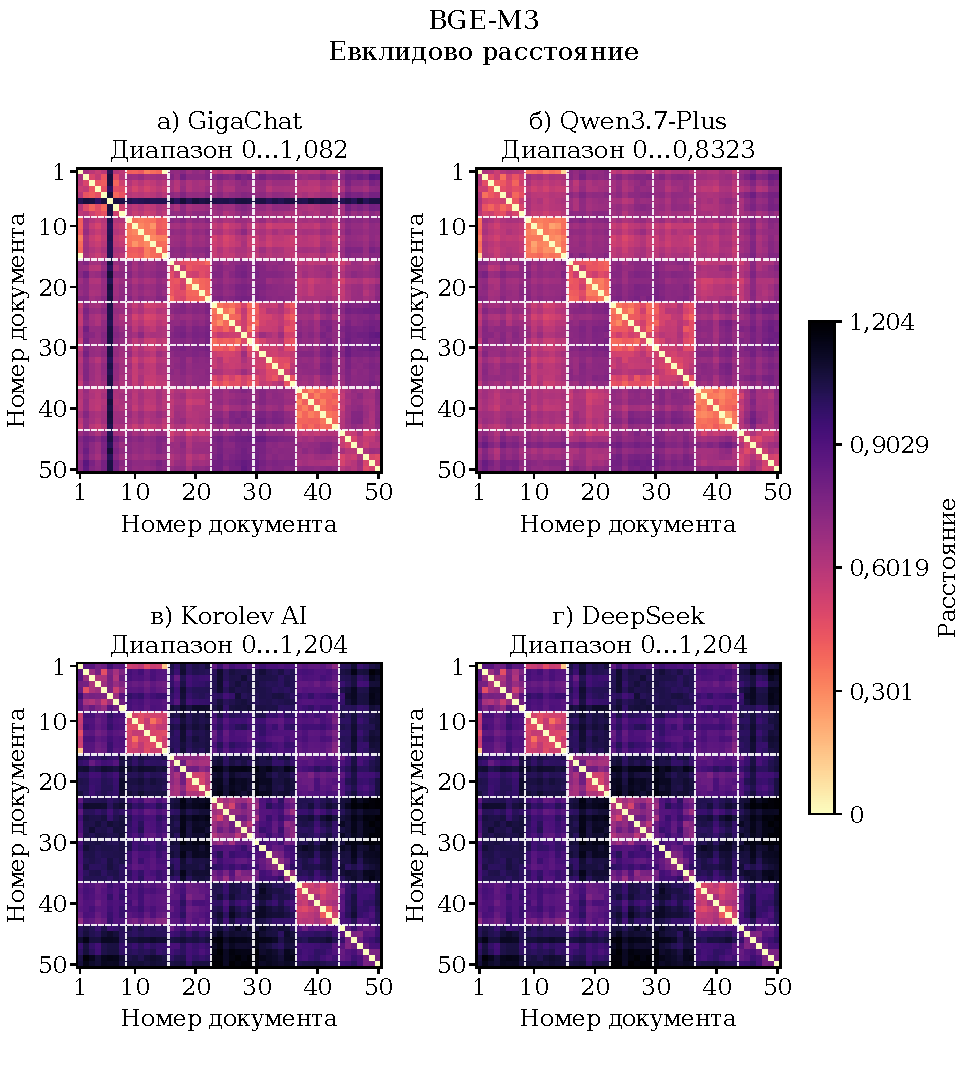
\includegraphics[width=\linewidth,height=0.78\textheight,keepaspectratio]{comparison_bge_m3_euclidean.pdf}
\caption{Евклидово расстояние для представления BGE-M3}
\label{fig:all-bge-m3-euclidean}
\end{figure}
\clearpage

Матрицы манхэттенского расстояния для данного представления приведены на рисунке~\ref{fig:all-bge-m3-manhattan}.

\begin{figure}[H]
\centering
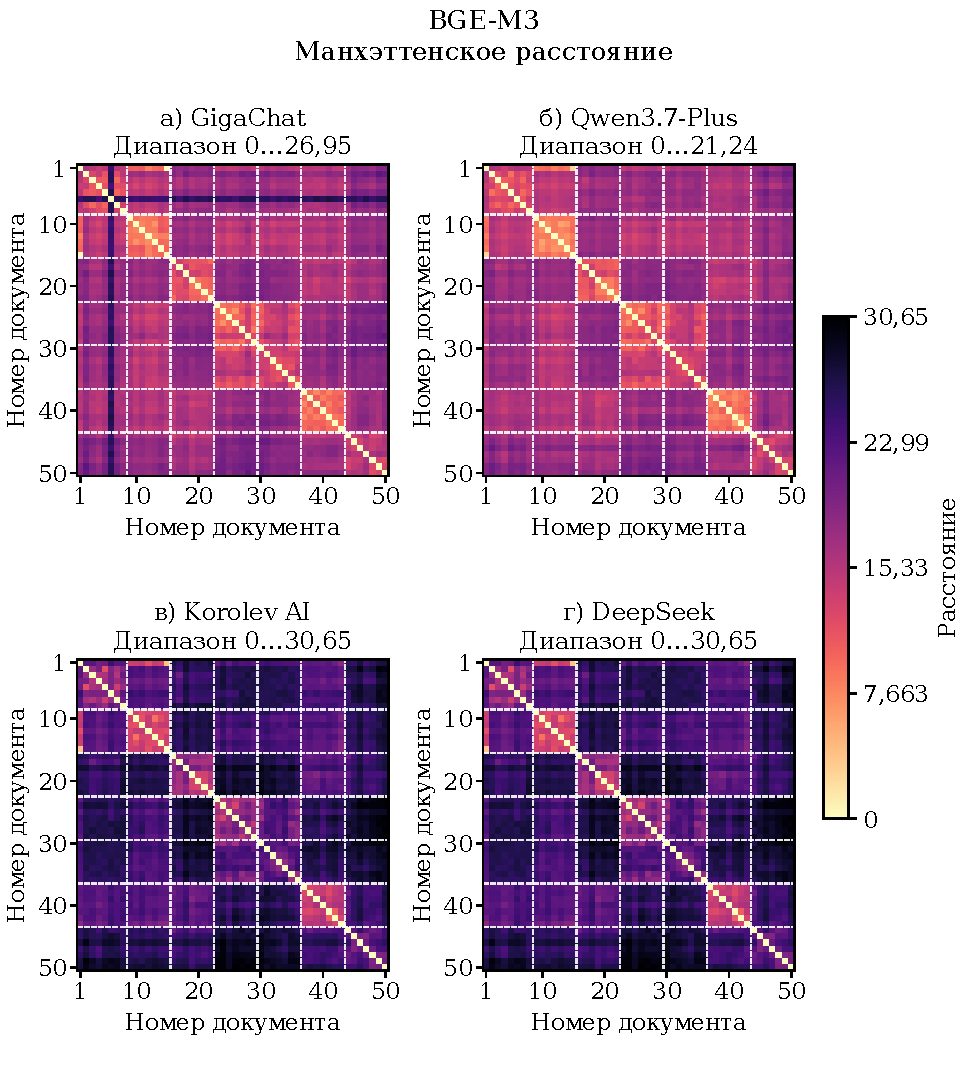
\includegraphics[width=\linewidth,height=0.78\textheight,keepaspectratio]{comparison_bge_m3_manhattan.pdf}
\caption{Манхэттенское расстояние для представления BGE-M3}
\label{fig:all-bge-m3-manhattan}
\end{figure}
\clearpage

Матрицы чебышёвского расстояния для данного представления приведены на рисунке~\ref{fig:all-bge-m3-chebyshev}.

\begin{figure}[H]
\centering
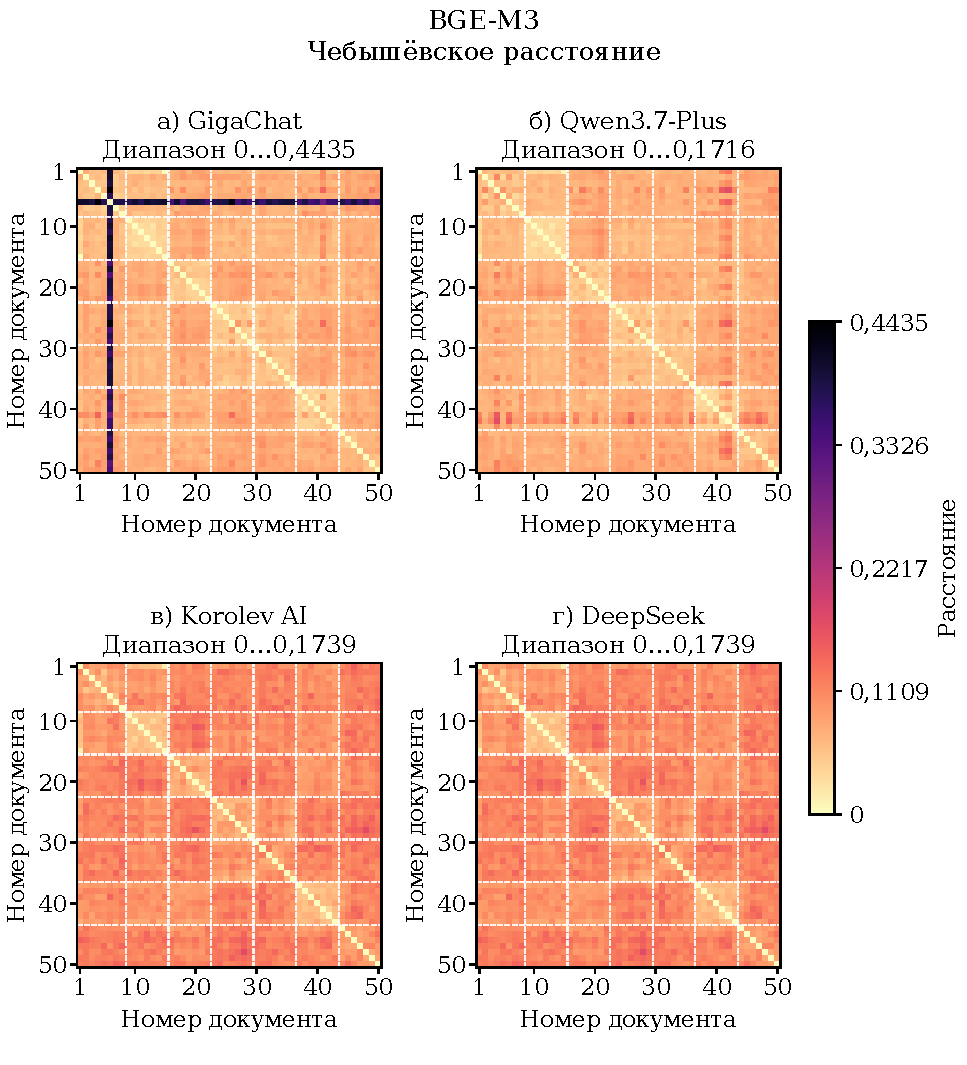
\includegraphics[width=\linewidth,height=0.78\textheight,keepaspectratio]{comparison_bge_m3_chebyshev.pdf}
\caption{Чебышёвское расстояние для представления BGE-M3}
\label{fig:all-bge-m3-chebyshev}
\end{figure}
\clearpage

Матрицы близости по евклидову расстоянию для данного представления приведены на рисунке~\ref{fig:all-bge-m3-euclidean-closeness}.

\begin{figure}[H]
\centering
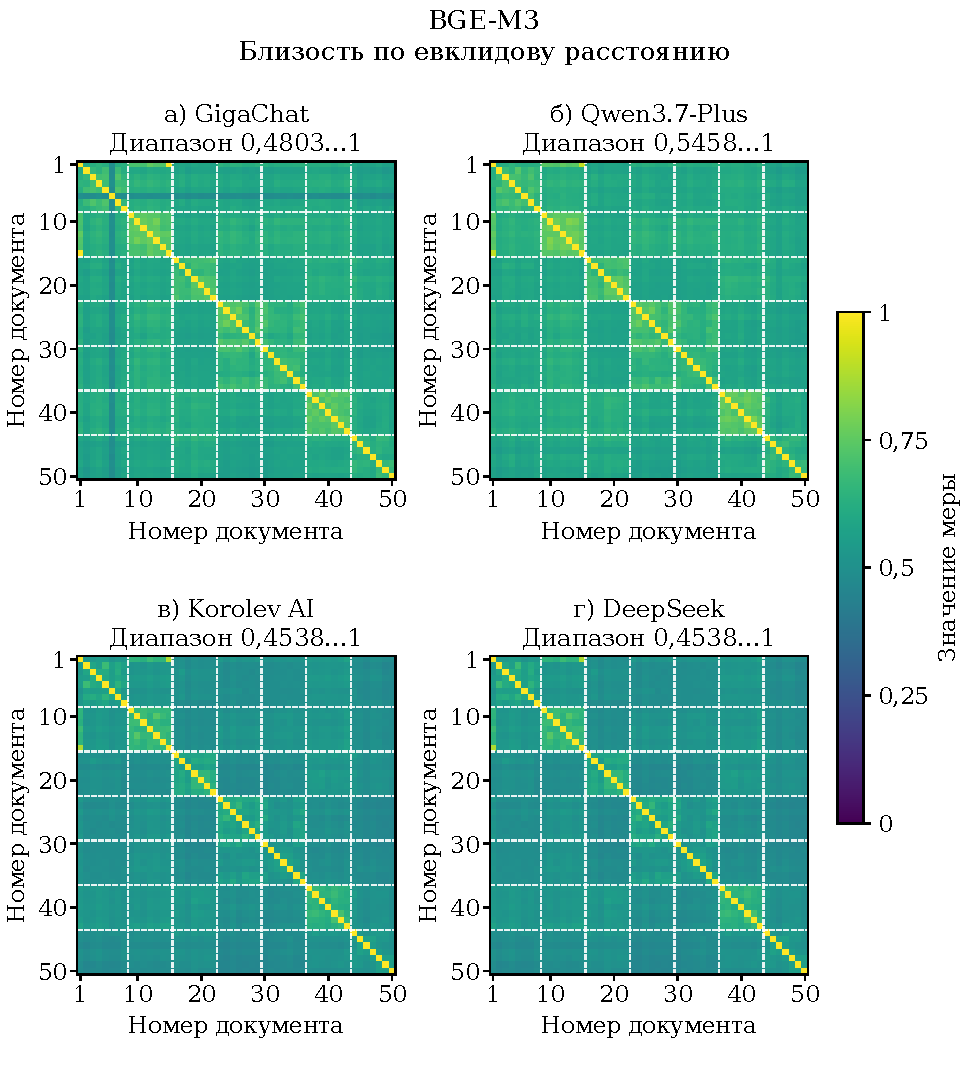
\includegraphics[width=\linewidth,height=0.78\textheight,keepaspectratio]{comparison_bge_m3_euclidean_closeness.pdf}
\caption{Близость по евклидову расстоянию для представления BGE-M3}
\label{fig:all-bge-m3-euclidean-closeness}
\end{figure}
\clearpage

Матрицы близости по манхэттенскому расстоянию для данного представления приведены на рисунке~\ref{fig:all-bge-m3-manhattan-closeness}.

\begin{figure}[H]
\centering
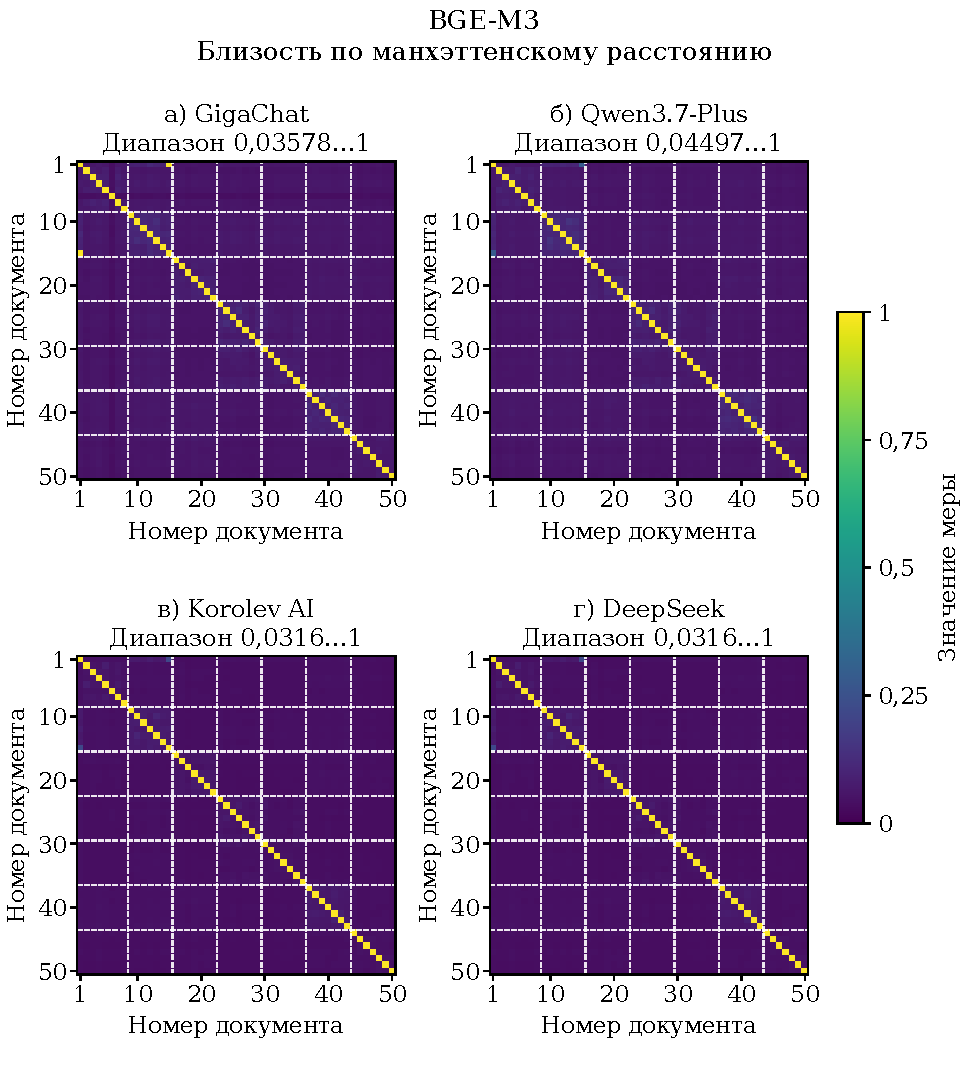
\includegraphics[width=\linewidth,height=0.78\textheight,keepaspectratio]{comparison_bge_m3_manhattan_closeness.pdf}
\caption{Близость по манхэттенскому расстоянию для представления BGE-M3}
\label{fig:all-bge-m3-manhattan-closeness}
\end{figure}
\clearpage

Матрицы близости по чебышёвскому расстоянию для данного представления приведены на рисунке~\ref{fig:all-bge-m3-chebyshev-closeness}.

\begin{figure}[H]
\centering
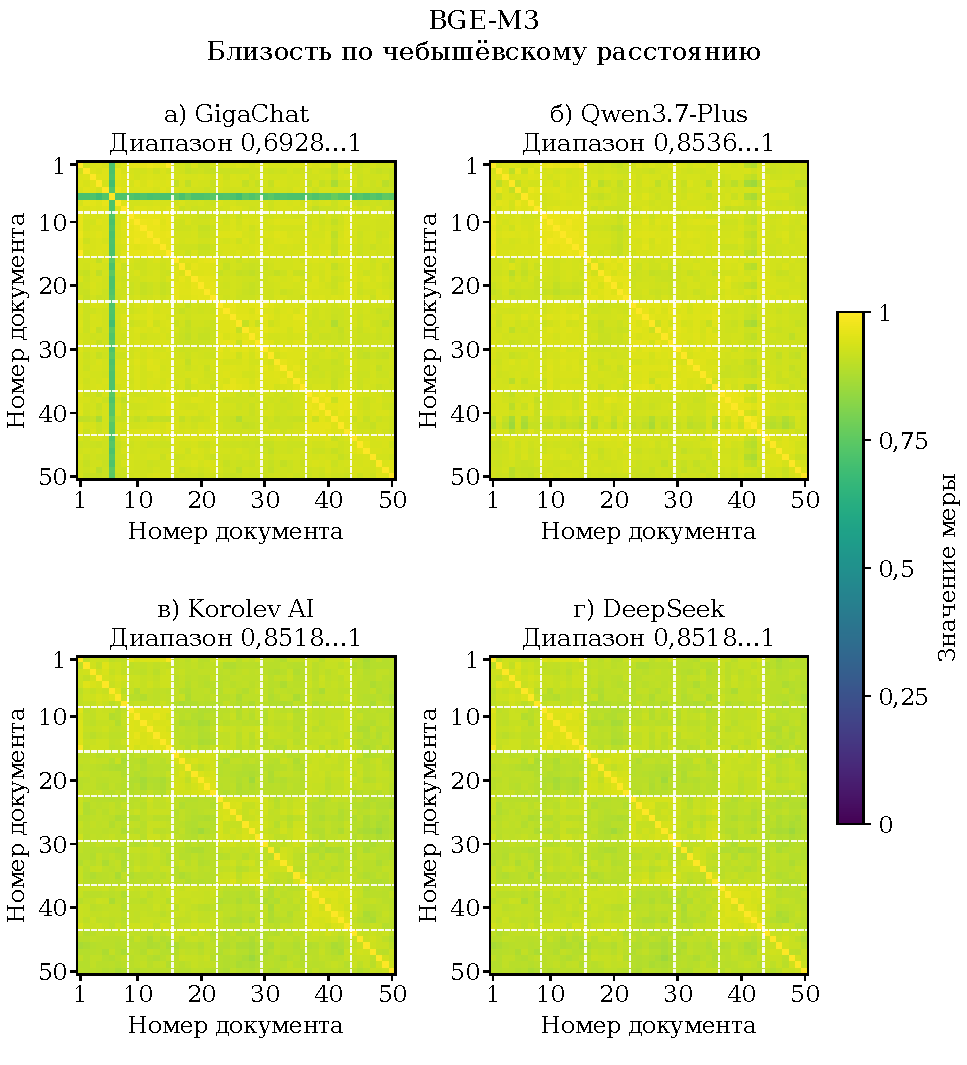
\includegraphics[width=\linewidth,height=0.78\textheight,keepaspectratio]{comparison_bge_m3_chebyshev_closeness.pdf}
\caption{Близость по чебышёвскому расстоянию для представления BGE-M3}
\label{fig:all-bge-m3-chebyshev-closeness}
\end{figure}
\clearpage

\section{Выводы по исследовательскому разделу}

Первый вывод состоит в том, что все четыре БЯМ способны сформировать сложный вычислительный конвейер, но результат необходимо проверять фактическим запуском. Ошибки, обнаруженные в эксперименте, не сводились к синтаксису: они затрагивали математическую интерпретацию, форматы данных и редкие ветви выполнения.

Второй вывод связан с полнотой тестов. Пустой каталог, два пустых документа и смешанный малый набор выявляли дефекты, которые могли не проявиться на полном корпусе. Проверки должны не только повторять основной сценарий, но и намеренно активировать вырожденные случаи.

Третий вывод относится к сравнению моделей. По числу ответов наиболее короткой оказалась цепочка DeepSeek, а максимальный ROC AUC и минимальное время финального запуска получены в реализации Qwen. GigaChat потребовал больше итераций, а Korolev AI занял промежуточное положение. Эти различия описывают данный эксперимент и не образуют универсального рейтинга сервисов.

Наконец, общий исходный запрос не приводит к идентичным программам. Модели по-разному реализовали токенизацию, агрегирование эмбеддингов, именование файлов и обработку граничных случаев. Поэтому сравнение должно учитывать не только наличие требуемых артефактов, но и воспроизводимость точной методики.

\section{Стабильность исправлений и ограничения исследования}

\subsection{Методика анализа стабильности}

После каждого исправления повторялись все ранее пройденные сценарии. Это позволило обнаруживать регрессии вне непосредственно изменённой ветви. Версия считалась устойчивой, если устраняла указанный дефект, сохраняла интерфейс командной строки и воспроизводила полный набор выходных файлов.

Особенно показателен signed-split. Одного правильного пояснения было недостаточно: требовалось проверить наличие преобразования именно в ветви Жаккара и Дайса, размерность конкатенации и диапазоны итоговых матриц. Такой контроль отделяет декларативное понимание от работающей реализации.

\subsection{Роль автоматической и визуальной проверки}

Основная проверка в данной работе была автоматической, поскольку результатом являлся числовой программный комплекс. Валидатор контролировал структуру файлов и инварианты значений. Визуальная проверка применялась к тепловым картам: изображения должны были открываться, содержать квадратные матрицы и отражать тот же порядок документов, что и CSV.

График сам по себе не доказывает корректность вычислений. Блочная структура может выглядеть правдоподобно даже при неверной нормировке. Поэтому визуализация использовалась после числовой проверки, как средство интерпретации, а не как замена тестам.

\subsection{Границы применимости результатов}

Исследована одна постановка, один корпус и одна цепочка ответов для каждой модели. Независимые повторные генерации не выполнялись, поэтому результаты не позволяют оценить статистическую вариативность БЯМ. Версии онлайн-сервисов могут изменяться, а повторение эксперимента позднее способно дать другую реализацию.

Тематическая метка каталога использовалась как приближённый эталон близости. Она не учитывает частичное пересечение тем и смысловые отношения между отдельными документами. ROC AUC показывает разделимость заданных групп, но не является исчерпывающей оценкой качества поиска похожих текстов.

Различия словарей показывают, что исходный запрос оставил свободу в деталях очистки. Для строгого сравнения алгоритмов следовало бы фиксировать единый токенизатор и единый набор признаков, а затем сравнивать только матричные операции. В настоящей работе, напротив, оценивается способность модели самостоятельно создать полный комплекс, поэтому такая вариативность является частью результата.

Наконец, время ответа онлайн-сервисов систематически не измерялось. Зафиксированы число итераций и время запуска финального кода, но не продолжительность генерации каждого ответа и ручной перенос в среду выполнения. Следовательно, выводы о трудоёмкости опираются прежде всего на структуру цепочки и характер исправлений.

\clearpage
\chapter*{ЗАКЛЮЧЕНИЕ}
\addcontentsline{toc}{chapter}{ЗАКЛЮЧЕНИЕ}

В работе исследована способность GigaChat, Qwen3.7-Plus, Korolev AI и DeepSeek создавать воспроизводимую систему попарного сравнения текстовых документов. Для каждой модели требовалось получить программу на Python, которая читает четыре формата, строит три представления, рассчитывает одиннадцать мер, сохраняет 33 матрицы и формирует аналитические артефакты.

Поставленная цель достигнута: получены и проверены четыре независимые реализации. Каждая финальная версия обработала 50 документов, создала полный набор матриц и прошла сценарии пустого, вырожденного, малого и полного корпуса. Взвешенные коэффициенты для знаковых BGE-M3 после преобразования находились в диапазоне $[0;1]$, а длинные таблицы содержали ожидаемые 40425 строк.

Ни один первоначальный ответ не удовлетворил всем требованиям. GigaChat был принят на шестой итерации, Qwen3.7-Plus и Korolev AI --- на четвёртой, DeepSeek --- на третьей. Следовательно, даже подробная постановка не устраняет необходимость цикла запуска, диагностики и исправления.

Наиболее короткую цепочку показал DeepSeek. Qwen сформировал реализацию с максимальным ROC AUC $0{,}953218$ и наименьшим временем полного запуска около 7,06~с. Korolev AI и DeepSeek получили близкие показатели BGE-M3, а GigaChat показал меньший максимум $0{,}915033$ и потребовал больше итераций. Эти значения характеризуют конкретные принятые программы, а не универсальные возможности моделей.

Главным методическим результатом является многоуровневая схема приёмки. Синтаксическая проверка должна предшествовать малым граничным тестам, а полный запуск --- завершаться контролем структуры, диапазонов и диагоналей. После любой правки необходимо повторять уже пройденные сценарии, поскольку исправление локального дефекта способно породить регрессию.

Эксперимент подтвердил важность точной математической обратной связи. Формулировка о некорректном диапазоне была преобразована в явное правило signed-split и ограничение области его применения. Только после проверки фактической вычислительной ветви исправление считалось выполненным. Аналогично ошибки ODT, пустого словаря и единственного класса устранялись надёжно лишь после предъявления воспроизводимого теста.

Организация работы через Codex сделала сравнение проверяемым. Исследуемые БЯМ создавали и исправляли реализации, Codex управлял проверками, формировал корректирующие запросы и принимал техническое решение о каждой версии по единым критериям. Пользователь участвовал в обмене с Korolev AI и оценивал соответствие результатов методике. Журналы приёмки позволяют проследить, какой дефект вызвал следующий запрос и на каком основании финальная версия была допущена к итоговому сравнению. Полученные результаты характеризуют модели в составе этого управляемого процесса.

\begin{samepage}
Перспективой дальнейшей работы является повторение эксперимента в нескольких независимых диалогах, фиксация времени генерации ответов, применение дополнительных корпусов и экспертная оценка ближайших соседей. Полезно также отделить вариативность предобработки от вариативности метрик, выполнив дополнительное сравнение четырёх программ на заранее сохранённых одинаковых векторах.
\par
\end{samepage}

\clearpage
\begin{thebibliography}{11}
\addcontentsline{toc}{chapter}{СПИСОК ИСПОЛЬЗОВАННЫХ ИСТОЧНИКОВ}
\bibitem{bge-m3} Chen J., Xiao S., Zhang P., Luo K., Lian D., Liu Z. BGE M3-Embedding: Multi-Lingual, Multi-Functionality, Multi-Granularity Text Embeddings Through Self-Knowledge Distillation // arXiv:2402.03216.~--- 2024.~--- URL: \url{https://arxiv.org/abs/2402.03216} (дата обращения: 18.11.2026).
\bibitem{gigachat} Руководства GigaChat API // Сбер~: документация для разработчиков.~--- URL: \url{https://developers.sber.ru/docs/ru/gigachat/guides/main} (дата обращения: 18.11.2026).
\bibitem{qwen} Qwen~: официальный репозиторий // GitHub.~--- URL: \url{https://github.com/QwenLM/Qwen} (дата обращения: 18.11.2026).
\bibitem{korolev} Королёв ИИ~: научно-образовательная платформа // МГТУ им.~Н.Э.~Баумана.~--- URL: \url{https://korolev-ai.bmstu.ru/} (дата обращения: 18.11.2026).
\bibitem{deepseek} DeepSeek~: официальный сайт.~--- URL: \url{https://www.deepseek.com/} (дата обращения: 18.11.2026).
\bibitem{sklearn} Pedregosa F., Varoquaux G., Gramfort A., et al. Scikit-learn: Machine Learning in Python // Journal of Machine Learning Research.~--- 2011.~--- Vol.~12.~--- P.~2825--2830.
\bibitem{pymorphy3} pymorphy3~: морфологический анализатор русского языка // GitHub.~--- URL: \url{https://github.com/no-plagiarism/pymorphy3} (дата обращения: 18.11.2026).
\bibitem{docx} python-docx~: documentation.~--- URL: \url{https://python-docx.readthedocs.io/} (дата обращения: 18.11.2026).
\bibitem{odfpy} odfpy~: Python API for OpenDocument Format // GitHub.~--- URL: \url{https://github.com/eea/odfpy} (дата обращения: 18.11.2026).
\bibitem{bs4} Beautiful Soup Documentation.~--- URL: \url{https://www.crummy.com/software/BeautifulSoup/bs4/doc/} (дата обращения: 18.11.2026).
\bibitem{transformers} Wolf T., Debut L., Sanh V., et al. Transformers: State-of-the-Art Natural Language Processing // Proceedings of the 2020 Conference on Empirical Methods in Natural Language Processing: System Demonstrations.~--- 2020.~--- P.~38--45.
\end{thebibliography}

\clearpage
\appendix
\renewcommand{\thechapter}{\Asbuk{chapter}}
\counterwithin{lstlisting}{chapter}
\renewcommand{\lstlistingname}{Листинг}

\gostappendix{Промты и ответы GigaChat}\label{app:gigachat}

Ниже в хронологическом порядке приведены исходный запрос, ответы модели и сохранённые корректирующие запросы. Принята итерация 06.

\logfile{GigaChat: исходный запрос}{../prompts/final_prompt_all_models.txt}
\logfile{GigaChat: ответ 01}{../models/gigachat/iterations/01/raw/response.txt}
\logfile{GigaChat: запрос после ответа 01}{../models/gigachat/iterations/02/correction_prompt.txt}
\logfile{GigaChat: ответ 02}{../models/gigachat/iterations/02/raw/response.txt}
\logfile{GigaChat: запрос после ответа 02}{../models/gigachat/iterations/03/correction_prompt.txt}
\logfile{GigaChat: ответ 03}{../models/gigachat/iterations/03/raw/response.txt}
\logfile{GigaChat: запрос после ответа 03}{../models/gigachat/iterations/04/correction_prompt.txt}
\logfile{GigaChat: ответ 04}{../models/gigachat/iterations/04/raw/response.txt}
\logfile{GigaChat: ответ 05}{../models/gigachat/iterations/05/raw/response.txt}
\logfile{GigaChat: ответ 06}{../models/gigachat/iterations/06/raw/response.txt}

\gostappendix{Промты и ответы Qwen3.7-Plus}\label{app:qwen}

Протокол включает четыре ответа. Третья версия содержала методическое пояснение signed-split, но требуемое преобразование появилось в рабочем коде только в итерации 04.

\logfile{Qwen3.7-Plus: исходный запрос}{../prompts/final_prompt_all_models.txt}
\logfile{Qwen3.7-Plus: ответ 01}{../models/qwen/iterations/01/raw/response.txt}
\logfile{Qwen3.7-Plus: запрос после ответа 01}{../models/qwen/iterations/02/correction_prompt.txt}
\logfile{Qwen3.7-Plus: ответ 02}{../models/qwen/iterations/02/raw/response.txt}
\logfile{Qwen3.7-Plus: запрос после ответа 02}{../models/qwen/iterations/03/correction_prompt.txt}
\logfile{Qwen3.7-Plus: ответ 03}{../models/qwen/iterations/03/raw/response.txt}
\logfile{Qwen3.7-Plus: ответ 04}{../models/qwen/iterations/04/raw/response.txt}

\gostappendix{Промты и ответы Korolev AI}\label{app:korolev}

Korolev AI взаимодействовал с пользователем вручную. Четвёртая итерация принята после исправления неопределённых AUC и average precision в одно-классовом сценарии.

\logfile{Korolev AI: исходный запрос}{../prompts/final_prompt_all_models.txt}
\logfile{Korolev AI: ответ 01}{../models/korolev-ai/iterations/01/raw/response.txt}
\logfile{Korolev AI: запрос после ответа 01}{../models/korolev-ai/iterations/02/correction_prompt.txt}
\logfile{Korolev AI: ответ 02}{../models/korolev-ai/iterations/02/raw/response.txt}
\logfile{Korolev AI: запрос после ответа 02}{../models/korolev-ai/iterations/03/correction_prompt.txt}
\logfile{Korolev AI: ответ 03}{../models/korolev-ai/iterations/03/raw/response.txt}
\logfile{Korolev AI: запрос после ответа 03}{../models/korolev-ai/iterations/04/correction_prompt.txt}
\logfile{Korolev AI: ответ 04}{../models/korolev-ai/iterations/04/raw/response.txt}

\gostappendix{Промты и ответы DeepSeek}\label{app:deepseek}

Ниже приведены три учитываемых ответа. Неполная копия ответа 02 не включена как отдельная итерация, поскольку возникла только из-за технического захвата уже начатого ответа.

\logfile{DeepSeek: исходный запрос}{../prompts/final_prompt_all_models.txt}
\logfile{DeepSeek: ответ 01}{../models/deepseek/iterations/01/raw/response.txt}
\logfile{DeepSeek: запрос после ответа 01}{../models/deepseek/iterations/02/correction_prompt.txt}
\logfile{DeepSeek: ответ 02}{../models/deepseek/iterations/02/raw/response.txt}
\logfile{DeepSeek: запрос после ответа 02}{../models/deepseek/iterations/03/correction_prompt.txt}
\logfile{DeepSeek: ответ 03}{../models/deepseek/iterations/03/raw/response.txt}

\gostappendix{Исходный код финальных решений}\label{app:code}

\lstinputlisting[style=logstyle,language=Python,caption={Финальная реализация GigaChat}]{../models/gigachat/final/solution.py}
\lstinputlisting[style=logstyle,language=Python,caption={Финальная реализация Qwen3.7-Plus}]{../models/qwen/final/solution.py}
\lstinputlisting[style=logstyle,language=Python,caption={Финальная реализация Korolev AI}]{../models/korolev-ai/final/solution.py}
\lstinputlisting[style=logstyle,language=Python,caption={Финальная реализация DeepSeek}]{../models/deepseek/final/solution.py}

\gostappendix{Состав электронного приложения}\label{app:electronic}

Электронное приложение содержит:

\begin{itemize}
\emergencystretch=1em
  \item единый исходный запрос и методическое дополнение signed-split в каталоге \code{prompts};
  \item неизменённые ответы моделей в каталогах \code{models/<model>/iterations/NN/raw};
  \item извлечённые программы, файлы зависимостей и отчёты проверок;
  \item корректирующие запросы для последовательных итераций;
  \item четыре принятые программы и результаты полного запуска в каталогах \code{models/<model>/final};
  \item общий валидатор структуры результатов \code{tests/verify_output.py};
  \item исходный корпус из 50 документов четырёх форматов;
  \item исходный текст настоящего отчёта и скомпилированный PDF-файл.
\end{itemize}

\end{document}
